\documentclass[a4paper,openany,titlepage]{book}

\usepackage[italian]{babel}
\usepackage[utf8]{inputenc}
\usepackage[T1]{fontenc}
\usepackage{amsmath}
\usepackage{mathtools}
%\usepackage{mathematics}
\usepackage{graphicx}
\usepackage{hyperref}
\usepackage{tikz}
\usepackage{amssymb}
\usepackage{mathrsfs}

\newcommand{\RNum}[1]{\uppercase\expandafter{\romannumeral #1\relax}}		%scrive i numeri romani
%\renewcommand{\openvir}{``}
%\renewcommand{'\closevir}{''  \,}
\renewcommand{\L}{\mathscr{L}}
\newcommand{\M}{\mathscr{M}}

\title{Introduzione all'astrofisica}

\begin{document}
\maketitle
\tableofcontents

%\toccontents

\chapter[Bertin-Panoramica]{Bertin-Panoramica generale dell'astrofisica moderna}

Il seguente estratto è preso dal primo volume del ``The Feynmann Lectures of Physics'', scritto nel 1963; l'argomento trattato è il cluster stellare noto con il nome $\omega$ Centauri, di cui sotto vengono riportate alcune specifiche:

\begin{figure}[h!]
\centering
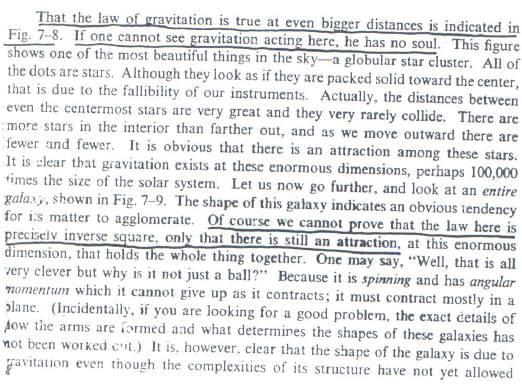
\includegraphics[width=1\textwidth]{Img/bertin_1.png}
\end{figure}

\clearpage
\begin{minipage}{.3\textwidth}
\centering
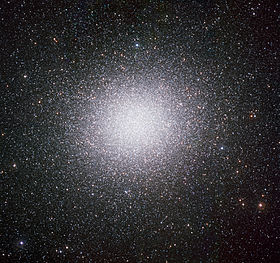
\includegraphics[width=1\textwidth]{Img/w_centauri.jpg}
\end{minipage}
\begin{minipage}{.65\textwidth}
\textbf{Cluster (ammasso stellare) $\omega$ Centauri}:
Distanza dalla Terra: circa 5 Kpc\footnote{Il parsec (pc) è l'unità di misura per le distanze stellari, e corrisponde a circa 3 anni luce.} , cioè circa 15000 anni luce.\\
Raggio del cluster: fra i 25 e i 50 pc.\\
Massa del cluster: $4 \cdot 10^6 \, M_\odot$ \footnote{$M_\odot$=massa solare~$2 \cdot 10^{33} \, kg$}.
\end{minipage}

\vspace{0.2cm}

Importante per lo studio di questi oggetti celesti è l'apporto dato da Henry Poincarè che, trattando un cluster stellare nel suo ``Science et Metode'' (1908), espose come il comportamento delle stelle all'interno del cluster fosse assimilabile al comportamento di un gas all'equilibrio termodinamico, poichè le stelle invece di scontrarsi riescono a seguire traiettorie che gli permettono di evitarsi a vicenda. Nella nostra galassia, la Via Lattea, sono finora stati contati 159 sistemi stellari di questo tipo.\\
\\
\begin{minipage}{.40\textwidth}
	\centering
	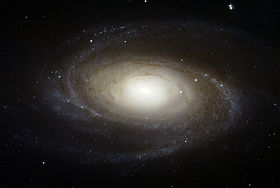
\includegraphics[width=.70\textwidth]{Img/M81_bis.jpg}
\end{minipage}
\begin{minipage}{.50\textwidth}
	Un'altro oggetto trattato nell'estratto riportato sopra è la galassia M81, nota come galassia di Bode, di cui viene riportata un immagine a lato.
\end{minipage}

\vspace{0.5cm}

A questo punto, apriamo una parentesi sulla nomenclatura degli oggetti celesti: esistono due cataloghi:
\begin{itemize}
	\item \textbf{Catalogo di Messier}: in questo catalogo, compilato dall'astronomo francese Charles Messier, vengono nominati ``solo'' 110 oggetti celesti (i più luminosi), ed è utilizzato soprattutto dagli astronomi non professionisti; la nomenclatura è formata da un numero tra 1 e 110 preceduto dalla lettera M.
	\item \textbf{Catalogo NGC (New General Catalogue)}: è il più famoso e usato catalogo di oggetti del profondo cielo nell'astronomia amatoriale; contiene circa 8000 oggetti ed è uno dei cataloghi più completi di tipo generale. Compilato da john Dreyer sulla base di ossevazioni condotte da William e John Herschel, associa agli oggetti celesti catalogati un numero fra 1 e 7840 preceduto dalla sigla NGC.
\end{itemize}
Per esempio, la galassia di Bode nei due cataloghi è chiamata rispettivamente M81 e NGC3031.

\section{Astronomia ottica}
Definiamo il \textbf{tempo dinamico} che caratterizza un sistema stellare la quantità $T=\frac{R}{v}$; possiamo anche costruire un tempo dinamico come:
$$\left[G \rho \right]=[T]^{-2} \rightarrow \left[ 4 \pi G \rho \right]=\left[T\right]^{-2} \rightarrow \sqrt{ \left[4 \pi G \rho \right]}=\left[ T \right]^{-1} \rightarrow T=\frac{1}{\sqrt{4 \pi G \rho}}$$
dove il fattore $4 \pi$ è legato all'equazione di Poisson.

Per fissare il concetto di tempo dinamico, utilizziamo un esperimento che possiamo trattare solo in via teorica (per evidenti limiti materiali);  immaginiamo di trivellare la Terra da una parte all'altra, in modo tale che il tunnel così ottenuto attraversi il centro del pianeta e sbuchi dalla parte opposta. A questo punto, lasciamo cadere un oggetto (dunque la velocità iniziale sarà nulla) all'interno del buco, in modo tale che tale oggetto non si scontri con le pareti durante il suo tragitto; noteremo che si instaurerà un moto oscillatorio dell'oggetto fra le due estremità del buco con una frequenza pari a $\sqrt{4 \pi G \rho}$.

Dal tempo dinamico, confrontato con il quadrato del parametro di Hubble $H_0 \left[Hz \right]$, possiamo inoltre capire se l'universo è aperto o chiuso, secondo la formula $\frac{H_0 ^2}{4 \pi G \langle \rho \rangle}$, dove $\langle \rho \rangle$ rappresenta la densità media dell'universo.
\\
\\
\textbf{Nota: dimensioni delle distanze stellari}\\
\textit{Nel parlare degli oggetti celesti, ci riferiremo spesso alla loro distanza reciproca dal punto di vista della superficie terreste; tali distanze saranno espresse in primo e secondi d'arco. Per farci un idea delle dimensioni che andiamo a trattare, un primo d'arco corrisponde al diametro apparente di Giove, mentre un secondo d'arco corrisponde al diametro apparente di una delle sue lune.}
\\
\\
Nel 1600 l'astronomo olandese Roemer, attraverso l'osservazione delle lune di Giove, riuscì a misurare con buona approssimazione la velocità della luce.
\\
\\
Per molto tempo si è posto l'accento sul miglioramento della capacità visiva tramite l'evoluzione dei telescopi ottici; da circa un secolo, siamo riusciti ad estendere il campo di osservazione a bande dello spettro elettromagnetico completamente diverse dalla classica fascia del visibile. Tradizionalmente, tali bande vengono denominate con le lettere:
\begin{itemize}
	\item \textbf{Radiazione $\gamma$}: corrisponde alle lunghezze d'onda fino a $1$ \AA$=1 \cdot 10*{-10} m$, ed è associata ad energie nell'ordine dei $MeV$.
	\item \textbf{Radiazione X}: corrisponde alle lunghezze d'onda da $1$ \AA \, fino ai $100$ \AA ($10^{-10}-10^{-8} \, m$), ed è associata ad energie nell'ordine dei $KeV$.
	\item \textbf{Radiazione Ultravioletta (UV)}: corrisponde alle lunghezze d'onda da $100$ \AA \, fino a $4000$ \AA ($10^{-8}-4 \cdot 10^{-8} \, m$).
	\item \textbf{Radiazione visibile}: la luce fascia che il nostro occhio riesce a percepire; corrisponde alle lunghezze d'onda da $4000$ \AA \, fino a $7000$ \AA ($4 \cdot 10^{-8}-7 \cdot 10^{-8} \, m$).
	\item \textbf{Radiazione Infrarossa (IR)}: corrisponde alle lunghezze d'onda da $7000$ \AA \, fino a $100 \mu m$ ($7 \cdot 10^{-8}-10^{-4} \, m$); possiamo distinguere fra due tipi di radiazione infrarossa: l'infrarosso vicino, per lunghezze d'onda di circa $1 \, \mu m$, e l'infrarosso lontano, per lunghezze d'onda dai $60 \, \mu m$ in su.
	\item \textbf{Radiazione Radio}: corrisponde alle lunghezze d'onda oltre i $100 \, \mu m$ ($10^{-4} \, m$). 
\end{itemize}
Questo fatto ha aperto gli occhi su un universo completamente nuovo; nonostante il campo di osservazione sia stato esteso, il ruolo della radiazione visibile rimane predominante a causa di un privilegio insito a quella fascia di lunghezze d'onda e riconducibile alla trasparenza dell'aria.
\\
\begin{minipage}{.50\textwidth}
	\centering
	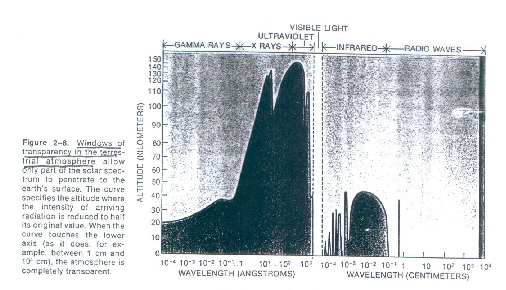
\includegraphics[width=1\textwidth]{Img/bertin_2.png}
\end{minipage}
\begin{minipage}{.50\textwidth}
	Nel grafico a fianco, vediamo ciò che abbiamo appena definito ``privilegio insito'' della radiazione visibile; la linea di demarcazione fra la zona più scura e la zona più chiara del grafico indica, alla lunghezza d'onda corrispondete (asse delle ascisse) l'altezza in $km$ (asse delle ordinate) alla quale il segnale proveniente dall'esterno viene dimezzato di intensità.
\end{minipage}
\vspace{0.3cm}
Notiamo tre cose: la prima è che, come avevamo detto, la luce nella fascia del visibile non viene smorzata dall'atmosfera, cosa che ne facilita la ricezione (a patto di mettersi nelle condizioni ottimali per l'osservazione, come spiegheremo in seguito); il secondo fatto che notiamo è che nella fascia del vicino infrarosso il grafico presenta molte gobbe: questo  fenomeno è oggetto di studio dell'astrofisica moderna (dal 1990 in poi).\\
Infine, notiamo come anche le onde radio non presentino smorzamenti del segnale, segno che la loro trasmissione è buona; questo permette agli astrofisici, diversamente da quanto succede per i telescopi ottici, di poter potenzialmente mettere un telescopio radio ovunque: infatti, mentre i telescopi ottici vengono in genere posti su alture e in luoghi molto secchi per evitare che le condizioni climatiche modifichino la misura, i telescopi radio non subiscono modifiche del segnale a causa delle condizioni metereologiche, e quindi ad esempio troviamo molti telescopi in Olanda, dove spesso piove.

L'astrofisico ha diverse fonti di informazioni per i suoi studi (in generale, tutto ciò che ci arriva dall'esterno risulta essere utile); principalmente vengono utilizzati i \textbf{raggi cosmici}, spesso chiamati anche raggi $\gamma$, e i neutrini.
\vspace{0.2cm}
\begin{minipage}{.50\textwidth}
	\centering
	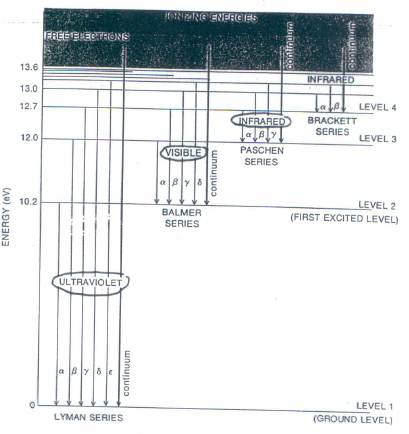
\includegraphics[width=1\textwidth]{Img/bertin_3.png}
\end{minipage}
\begin{minipage}{.50\textwidth}
	Un ruolo chiave nello studio astrofisico lo gioca l'atomo di idrogeno, i cui livelli di energia sono riportati nel grafico a fianco; infatti le righe di assorbimento che si ottengono nelle osservazioni sono spesso riconducibili allo spettro di assorbimento dell'idrogeno, presente in gran quantità sotto forma atomica (più che come ione $H_2$).\\
	In particolare, ci soffermiamo su quella che è chiamata \textbf{serie di Balmer}: infatti, a causa del salto energetico che compiono gli elettroni, facendo sì che queste transizioni (in particolare le $H \alpha$ e $H \beta$) giochino un ruolo essenziale nell'astronomia ottica.
\end{minipage}
\clearpage
\begin{minipage}{.45\textwidth}
Un'altro grafico interessante è quello riportato qui a fianco, in cui leggiamo i valori della capacità di trasmissione dell'aria (e quindi dell'atmosfera) per fotoni nella regione del vicino infrarosso (qualche $\mu m$); notiamo che ci sono tre regioni, denominate con le lettere J, H, K, per le quali il valore della trasmissione è molto alto: questo ci indica che, per le lunghezze d'onda relative a tali regioni, la trasmissione dei fotoni da parte dell'atmosfera è pressocchè totale, e dunque l'osservazioni in tali finestre è molto facilitata.
\end{minipage}
\begin{minipage}{.55\textwidth}
	\centering
	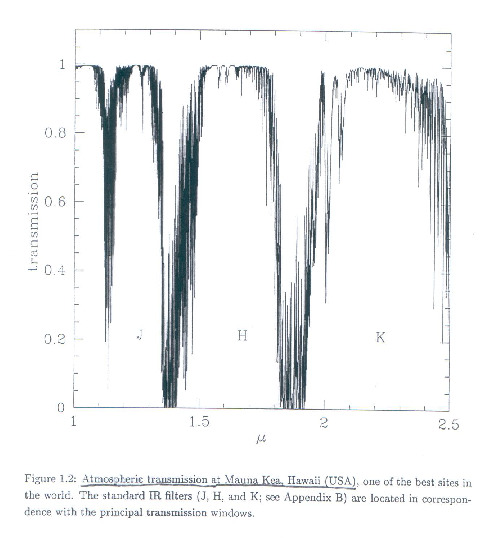
\includegraphics[width=1\textwidth]{Img/bertin_4.png}
\end{minipage}

\vspace{0.2cm}

A questo punto, ha senso riprendere in mano il discorso introdotto precedentemente sugli strumenti di osservazione, e in particolare parlare in maniera più estesa dei telescopi nell'ottico-infrarosso. Il telescopio  più grande su suolo europeo si trova sul Caucaso e ha un diametro primario di $6 \, m$; ma non è il più grande al modo: questo primato appartiene ai due telescopi Keck\footnote{Non è vero, esiste il Gran Telescopio Canarias che ha un diametro di $10,4 \, m$ e si trova su una montagna dell'isola di La Palma, nelle isole Canarie (ma va!!!). Non so se è un errore di Bertin oppure se ho capito male io, nel dubbio lo lascio così che fa scena.} (dal nome dell'imprenditore americano che ne finanziò la costruzione) con un diametro primario di $10 \, m$ ciascuno. Questi ultimi sono stati posti sulla sommità del vulcano (spento) Mauna Kea, nelle isole Hawaii, e sono costituiti da segmenti esagonali posti uno di fianco all'altro. Infine, un'altro telescopio degno di nota è il Very Large Telescope (VLT), posto sulle alture del Cile e di proprietà dell'ESO; la particolarità di questo telescopio sta nel fatto di essere costituito da quattro telescopi, ognuno di diametro principale di $6 \, m$.

Notiamo che, come avevamo già accennato in precedenza, tutti questi telescopi ottici sono posti molto in alto e in luoghi generalmente deserti: questo infatti permette di minimizzare gli effetti dovuti all'assorbimento della Terra (in particolare del vapor d'acqua), che altrimenti nasconderebbe la radiazione infrarossa; inoltre i telescopi vengono tenuti al freddo (o comunque a temperature prossime a quelle locali), in modo tale da evitare che il calore irradiato dagli edifici vada a modificare e rovinare le osservazioni.
\\

A questo punto, risulta  naturale trattare gli oggetti osservati con la strumentazione fin qui esposta, e la prima cosa a cui si pensa è il cielo stellato; in estate, se le condizioni atmosferiche lo permettono e l'inquinamento luminoso non è elevato, si può notare in cielo una striscia con una maggior concentrazione di stelle, uno dei bracci della Via Lattea (più precisamente, quello in cui si trova il nostro sistema solare). Si nota inoltre che tale fascia di cielo non è coperta uniformemente dalle stelle, ma intervalla zone luminose a zone scure, molte delle quali sono permanenti (e quindi non dovute alle condizioni atmosferiche): questo fenomeno è dovuto dal fatto che, essendo all'interno di una galassia, il piano del disco\footnote{Dimensioni del ``disco'' che modellizza la galassia: $500 \, pc$ di altezza, $15 \, Kpc$ di raggio.} che è la Via Lattea viene riflesso e, dato che essa contiene molto mezzo interstellare (formato da gas, principalmente idrogeno, e polveri), si ha che tale mezzo interstellare fa molto assorbimento, generando figure di questo genere. Tale fenomeno si riscontra, in maniera diversa, anche nell'osservazione di altre galassie (ad esempio la già citata M81), sulle cui immagini si trovano delle ``strisciate'' più scure, dette \textbf{dust lanes}; oltre a questo inconveniente, però, le polveri sono molto utili agli astronomi nelle osservazioni nella regione del vicino infrarosso, poichè permettono di eliminare un po di ``sporcizia'' dalle immagini. Guardando dei fuochi d'artificio, sappiamo che la massa è poca rapportata alla luminosità prodotta; ci chiediamo allora se, nel caso delle dust lanes,  il processo sia lo stesso, cioè se questi fenomeni siano generati da oggetti molto massivi o meno. Questo apre al problema della distribuzione della massa nell'universo.
%In ogni caso, la domanda che ci si pone è se tali figure siano fisse oppure se siano solo ``di passaggio'', e dunque si pone il problema, tutt'oggi oggetto di studio, della distribuzione della massa nell'universo.
\\
La maggior parte della massa (in stelle) nelle galassie risulta essere distribuita fra supergiganti o stelle fredde, le quali emettono soprattutto nella fascia del vicino infrarosso; questo ci fa dunque capire l'importanza delle osservazioni che riguardano tale radiazione.
\\
\\
\textbf{Nota: misura della magnitudine}\\
\textit{L'assorbimento della luce si misura in magnitudini; il valore di una magnitudine si ricava dalla formula:
$$[mag]=-2.5 \cdot Log(I)$$
dove $I$ è l'intensità del flusso luminoso (tutte le misure hanno sempre un oggetto di riferimento, e dunque avremo che $[mag]=[mag]_x - [mag]_0$ e $I=\frac{I_x}{I_0}$). Ad esempio, un assorbimento di 30 magnitudini equivale a fare $(10^2)^6$, poichè si ha che $2,5 \cdot Log(10^{12})=2,5 \cdot 12=30$, e dunque l'intensità del flusso luminoso assorbita è pari a $10^{12}$.}
\\
\\
Oltre al discorso sulla massa, sappiamo che l'universo è in espansione e, a parte ciò che succede nell'universo vicino a noi (qualche decina di milione di parsec), andando sempre più in là si ha questa espansione che si fa sempre più accentuata; tale espansione è trattabile in termini cinematici, tramite l'effetto doppler: questo genera il fenomeno di \textbf{redshift}, cioè lo spostamento della lunghezza d'onda verso la fascia del rosso (lunghezze d'onda maggiori). Si parla di redshift degli oggetti celesti, e per ricavare il valore di tale grandezza si utilizza:
$$z=\frac{\Delta \lambda}{\lambda} \sim \frac{v}{c}\footnote{Attenzione! è stato ricavato un valore di redshift $z=11$, ma questo non vuol dire che $v=11 \cdot c$,  ma mi dice che la lunghezza d'onda dell'emissione è spostata di un fattore 11( e dunque $\frac{\Delta \lambda}{\lambda}=11$).}$$

\vspace{0.2cm}

Nel guardare le stelle (sia attraverso strumenti ottici sia a occhio nudo) notiamo che esse, invece di apparirci come dei punti luminosi nel cielo, hanno un certo ``sbrilluccichio'' che le fa assomigliare a dei brillantini; questo fenomeno è dovuto alla dimensione angolare delle stelle che fa sì che le turbolenze dell'atmosfera siano rese più visibili, generando appunto tale fenomeno. Però questo non accade per il pianeta Giove, che ci appare come un punto ben definito nel cielo; questo perchè Giove ha una dimensione angolare (1' d'arco) maggiore di un certo angolo caratteristico, chiamato \textbf{seeing}. Il seeing, in termini qualitativi, può essere descritto come un degrado dell'immagine; questo degrado può avvenire per sue fattori: il primo è la turbolenza dell'aria (che però è solitamente legato al basso cielo), il secondo è sintetizzabile dal termine errori ottici (diffrazione, distanza focale errata...).\\
L'azione della turbolenza dell'aria è quella di trasformare un punto (rappresentabile matematicamente tramite una $\delta(\vec{x})$) in una macchiolina (matematicamente una PSF\footnote{Per maggiori informazioni, visitare \url{https://en.wikipedia.org/wiki/Point_spread_function} (PSF), \url{https://en.wikipedia.org/wiki/Astronomical_seeing} (seeing)}, acronimo di Point Spread Function); in particolare, viene messo a repentaglio quello che viene chiamato \textbf{limite rifrattivo} $\theta \sim \frac{\lambda}{D}$, che rappresenta la miglior risoluzione angolare ottenibile. Per molto tempo si è cercato di ovviare a tale problema costruendo telescopi sempre più grandi, ma questo aiuta fino ad un certo punto nella regione del visibile, cioè aumentando le dimensioni del telescopio la risoluzione angolare migliora sempre meno. Per risolvere questo degradamento dell'immagine si utilizzano metodi di \textbf{ottica adattiva}, che consiste nel pulire le immagini dagli effetti del seeing tramite una calibrazione operata su altre stelle, dalle quali viene ricavata la PSF che poi viene utilizzata per risolvere l'immagine del corpo celeste che si sta osservando. In questo tempo, è stato avviato il progetto di costruzione del telescopio EELT (acronimo di European Extremely Large Telescope), un telescopio di $40 \, m$ che permetterà di eseguire sempre l'ottica adattiva, poichè la zona di cielo che può essere osservata avrà sempre abbastanza stelle per permettere questo processo.
%Funzione di green (suggerita, ma non so a che serve)
\\
\\
I telescopi hanno due modi per raccogliere informazioni:
\begin{itemize}
	\item \textbf{Imaging}: questo processo consiste nella raccolta di mappe di intensità della zona di osservazione, e viene spesso utilizzata per farsi un'idea della natura della sorgente partendo dalla sua massa; infatti, si parte dall'assunzione che la massa e l'intensità luminosa dell'oggetto in questione siano proporzionali, $m \propto I$. Dunque le informazioni che si ricavano tramite questo procedimento sono di tipo strutturali, poichè si ricava una prima idea di come sia distribuita la massa.
	\item \textbf{Spettroscopia}: anch'essa ha come oggetto di studio e di raccolta dati l'intensità luminosa, ma, diversamente dall'imaging, si va a studiare l'andamento dell'intensità in funzione della lunghezza d'onda; essa infatti da vita a due  figure, dette spettro di assorbimento e spettro di emissione. Da essi si ricavano due tipi di informazioni: la prima è un informazione di tipo \textbf{``chimico''}, poichè, a seconda delle righe dei due spettri possiamo ricavare la composizione chimica dell'oggetto osservato. La seconda informazione è di tipo \textbf{cinematico}, e sfrutta l'effetto doppler: infatti, come avevamo già visto in precedenza, conosciamo le righe degli spettri di emissione e di assorbimento dell'idrogeno e dunque, misurando le lunghezze d'onda di tali righe e confrontandole con le lunghezze d'onda ricavate tramite i calcoli, possiamo trovare il valore del redshift e quindi (fintanto che non siamo in regime relativistico) la velocità con cui si muove la stella e la sua direzione, tramite la formula già vista in precedenza:
	$$z=\frac{\Delta \lambda}{\lambda}=\frac{\lambda_o - \lambda_e}{\lambda_e} \sim \frac{v}{c}$$
	dove $\lambda_o$ rappresenta la lunghezza d'onda osservata mentre $\lambda_e$ è la lunghezza d'onda conosciuta (dello spettro di emissione). 
\end{itemize}

Però nel fare della spettroscopia si ha l'inconveniente del numero di fotoni richiesti, che è molto maggiore di quelli che servono per fare dell'imaging; questo apre al problema del fare dell'astronomia sulla Terra o nello spazio: in alcuni casi ci troviamo costretti a scegliere la seconda opzione (ad esempio, non è possibile costruire un ... del telescopio spaziale Hubble sulla Terra), in altri casi, come per esempio lo studio della regione del visibile, questo problema non si pone, e spesso conviene operare da terra per abbattere sensibilmente i costi (e i tempi) di manutenzione della strumentazione.

Nella pagina successiva possiamo vedere un esempio di caso in cui l'unica possibilità  sia quella di mandare la nostra strumentazione nello spazio.

\subsubsection{Note alla scheda}
Il telescopio spaziale Hubble occupa un orbita bassa (orbita ad un altezza di $500 \, km$ dalla superficie terrestre); questo permette, in caso di guasti, di poter intervenire in termini tutto sommato brevi, come è successo all'inizio della missione quando ci si accorse che la distanza focale era errata di $2 \, mm$; di contro, il fatto di essere in orbita così vicino alla Terra (compie un giro in un ora e mezza circa) rende molto difficile la raccolta di informazioni per l'imaging, poichè oltre al problema del puntamento che viene implementato tramite l'utilizzo di due giroscopi si ha che per metà della sua orbita il tratto di cielo sa osservare sarà coperto, e questo rende difficile la raccolta di dati. Le dimensioni del telescopio, inoltre, non permettono di fare della buona spettroscopia; dunque la'attività di raccolta dati si limita all'imaging, e le informazioni ricavate da questo processo vengono utilizzate per fare spettroscopia da terra con telescopi più grandi (ad esempio VLT, i due Keck...).\\
Invece il JWST (acronimo di James Webb Space Telescope) sarà posto a $1,5 \cdot 10^6 \, km$ dalla Terra, nel punto lagrangiano $L_2$ dove, come vedremo successivamente, è in equilibrio rispetto alla congiungente Terra-Sole, e  dunque seguirà la Terra nella sua orbita intorno al Sole. Il suo compito sarà non tanto quello di fare dell'imaging (cosa che verrà comunque svolta) ma piuttosto avrà il compito di fare della spettroscopia nella regione del vicino infrarosso; la gestione è affidata allo stesso ente che gestisce l'Hubble, lo Space Telescope Science Institute (STScI), che ha sede  Baltimora, e ha come capo missione Massimo Stiavelli. Sarà più grande del suo predecessore (il telescopio Hubble ha un diametro di $2,4 \, m$); per poterlo spedire in orbita senza rovinare la strumentazione, verrà utilizzato un processo di apertura ``ad ombrello''.\\
L'anno previsto per il lancio del telescopio è il 2018; in basso a sinistra della scheda sono riportati i principali obbiettivi della missione.

\clearpage

\begin{tikzpicture}[remember picture,overlay] 
\pgfdeclareimage[width=\paperwidth]{image}{Img/bertin_5.jpg}
\node at (current page.center) {\pgfuseimage{image}}; 
\end{tikzpicture}

\clearpage

Abbiamo detto che il JWST verrà posto a $1,5 \cdot 10^6 \, km$ dalla Terra, nel punto $L_2$; questo punto fa parte di un insieme di punti, detti \textbf{punti lagrangiani}, in cui si verificano particolari condizioni di equilibrio.
\vspace{0.05cm}
\\
\begin{minipage}{.55\textwidth}
Nonostante il nome, si deve la scoperta di tali punti (riportati nell'immagine a lato) ad Eulero, che per primo di pose il problema della ricerca di punti in cui si avesse equilibrio fra le forze gravitazionali dovute alla Terra e al Sole e la forza centripeta (dovuta al moto orbitale degli oggetti); risolvendo il problema corrispondente, tradizionalmente detto \textbf{problema dei tre corpi ristretto}, Eulero ricavò la posizione dei punti $L_1$, $L_2$ e $L_3$ (quelli sulla congiungente Terra-Sole).
\end{minipage}
\begin{minipage}{.40\textwidth}
	\centering
	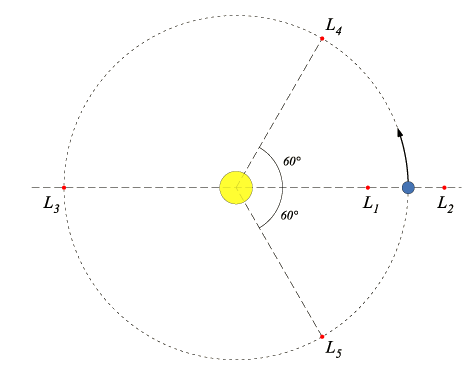
\includegraphics[width=1\textwidth]{Img/pti_lagrangiani_bis.png}
\end{minipage}
\vspace{0.1cm}
\\
\begin{minipage}{.35\textwidth}
	\centering
	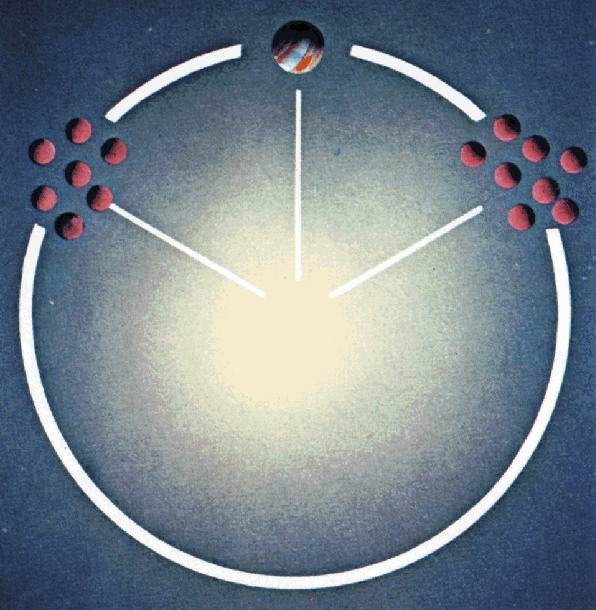
\includegraphics[width=1\textwidth]{Img/pti_lagrangiani_giove.jpg}
\end{minipage}
\begin{minipage}{.65\textwidth}
Successivamente, Lagrange mise mano allo stesso problema e ricavò i punti $L_4$ e $L_5$ (quelli sull'orbita terrestre): l'esistenza di questi ultimi fu poi confermata da osservazioni inerenti l'orbita di Giove, sulla quale vennero osservati due gruppi di asteroidi\footnote{Questi due gruppi di asteroidi si trovano fuori dalla fascia degli asteroidi del nostro sistema solare e sono chiamati Troiani e Greci, perchè, essendo sui due punti $L_4$ e $L_5$, proprio come i troiani e i greci si rincorrono senza mai scontrarsi.} proprio in corrispondenza di tali punti.
\end{minipage}
\vspace{0.05cm}

La natura di questi punti però non è uguale: infatti abbiamo che i punti $L_1$, $L_2$ e $L_3$ sono punti di equilibrio instabili, mentre $L_4$ e $L_5$ sono punti di equilibrio stabili; al di là della dimostrazione matematica, possiamo mostrare che questa conclusione è ragionevole semplicemente ragionando sulle forze coinvolte: se ad esempio ci mettiamo su $L_2$, possiamo facilmente vedere che, spostandoci di poco a destra (verso la Terra) o a sinistra (allontanandoci dalla Terra) prende il sopravvento rispettivamente la forza di gravità combinata del sistema Terra-Sole e la forza centripeta, facendo quindi allontanare ulteriormente il nostro oggetto dal punto di equilibrio. Il ragionamento per $L_1$ e $L_3$ è simile.\\
Invece per dimostrare che $L_4$ e $L_5$ sono punti di equilibrio stabili ci tocca risolvere le equazioni del problema a tre corpi; quello che abbiamo appena descritto è riassunto nell'immagine qua sotto.

\begin{figure}[h!]
	\centering
	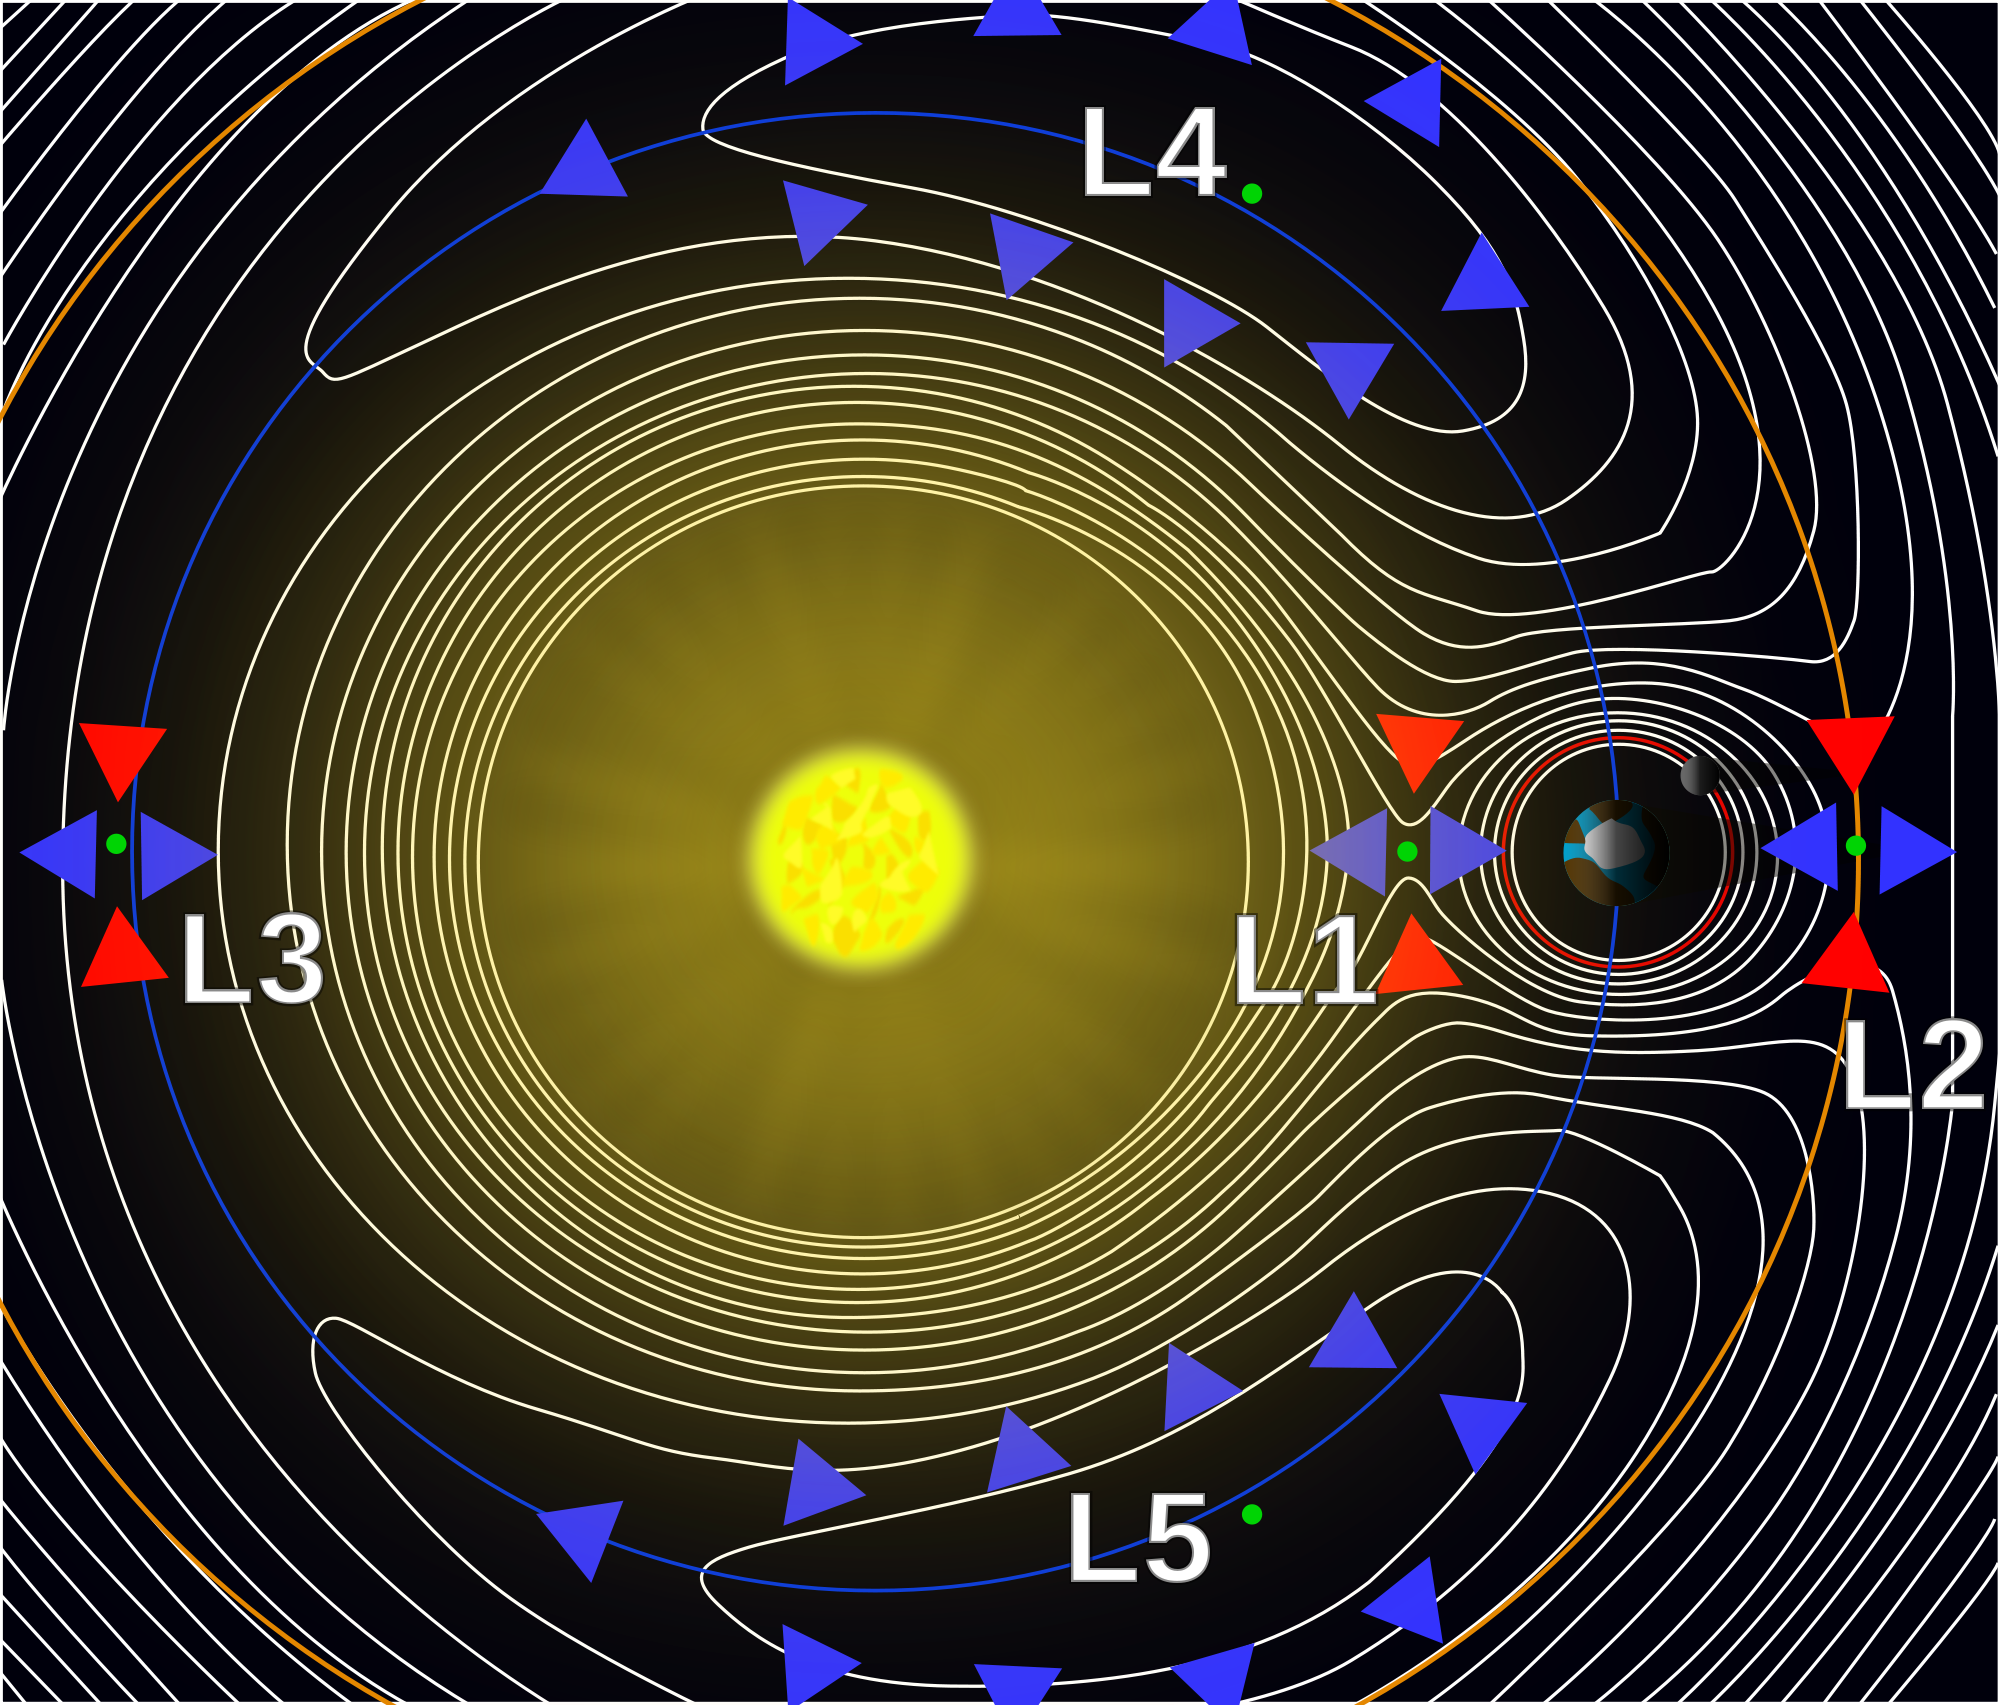
\includegraphics[width=0.45\textwidth]{Img/pti_lagrangiani_grafico.png}
\end{figure}

Detta $r$ la distanza della massa minore (nel nostro caso, la Terra) dal punto $L_2$ e $R$ la distanza fra i due corpi massivi (per noi sarà la distanza Terra-Sole), abbiamo che il rapporto $\frac{r}{R}$ scalerà come una potenza di $\frac{m}{M}$, dove $m$ e $M$ sono le due masse considerate; in particolare, avremo che $\frac{r}{R} \approx \left( \frac{m}{M} \right) ^{\frac{1}{3}}$.\\
Il fatto che il valore dell'esponente sia $\frac{1}{3}$ ci sembra strano, poichè eguagliando le due espressioni delle forze gravitazionali (per cui mettendoci nella condizione di equilibrio) si otterrebbe $\frac{1}{2}$; ragionando in questo modo però si fa un errore, perchè si ignora la forza centripeta, e il bilancio delle forza è:
$$\frac{GMm_o}{(R+r)^2} + \frac{Gmm_o}{r^2} - \Omega^2(R+r)$$
Operando un espansione del primo termine, vediamo che effettivamente ci rimane un termine del tipo $\frac{r}{R^3}$ (gli altri termini si eliminano con il termine di forza centripeta) e il termine di forza di gravità della Terra; ponendo tutto uguale a zero si ha la condizione cercata.
\\
\\
Infine, nella pagina successiva troviamo alcuni importanti progetti in diversa fase realizzativa di telescopi che operino nella regione dell'infrarosso.

\subsubsection{Note alla scheda}
\textbf{ALMA}
\\
Acronimo di Atacama Large Millimeter/submillimeter Array, è un complesso di antenne  che lavoreranno in modo interferometrico; il fronte d'onda raccolto dalle varie antenne viene sottoposto ad un processo di combinazione elettronica, il che permette di gestire una porzione di cielo molto più grande di quanto non sia possibile con una sola antenna (si parla di interferometria). La distanza tra le antenne va dai $150 \, m$ ai $16 \, km$; avere antenne che lavorano in modo interferometrico a tali distanze permette, entro certi limiti, di migliorare la risoluzione angolare, e infatti si può ottenere una risoluzione angolare di $0,005$ secodni d'arco. Il rischio che comporta lavorare in questa maniera è quello di non avere abbastanza fotoni radio,e dunque nell'impostare un esperimento del genere bisogna porre particolare attenzione alla sensibilità richiesta e ottenibile.
\\
\\
\textbf{SKA}\\
In fase di costruzione, è anch'esso un complesso di antenne, divise fra Sud Africa e Australia, che raggiungeranno una superficie ``di assorbimento'' di un kilometro quadrato (Square Kilometre Array).
\\
\\
Tutti i telescopi radio visti sono formati da più unità che lavorano interferometricamente; esistono però anche dei radiotelescopi a piatto unico con dimensioni paragonabili a questi complessi. Il più grande e il più famoso si trova as Arecibo, nell'isola caraibica di Porto Rico, e ha un diametro di $300 \, m$. Questo radiotelescopio è stato ricavato nella conca fra tre colline ed ha tre piloni che fungono da supporto per tenerlo sollevato da terra (ci si può passare sotto con una jeep); viste le dimensioni, questo radiotelescopio non è orientabile ma è fisso.\\
Il radiotelescopio a piatto unico orientabile  più grande al mondo è l'Effelsberg\footnote{Ne esiste uno in Virginia, il radiotelescopio di Green Bank, ed è più grande.}, in Germania, ed ha un diametro di circa $100 \, m$.


\clearpage

\begin{tikzpicture}[remember picture,overlay] 
\pgfdeclareimage[width=\paperwidth]{image}{Img/bertin_5bis.jpg}
\node at (current page.center) {\pgfuseimage{image}}; 
\end{tikzpicture}

\clearpage

\subsection{Campi profondi di Hubble}
Quando parliamo di campi profondi di Hubble parliamo di una serie di osservazioni compiute dal telescopio spaziale Hubble nei suoi vent'anni di servizio; distinguiamo tre diverse trance osservazioni:
\begin{itemize}
	\item \textbf{Hubble Deep Field} (HDF), 1995; a sua volta si divide in South e North
	\item \textbf{Hubble Ultra Deep Field} (HUDF), 2004; fu necessario un puntamento di undici giorni per ottenere l'immagine definitiva 
	\item \textbf{Hubble Xtremely Deep Field} (HXDF), 2012; fu necessario un puntamento di ventidue giorni per ottenere l'immagine definitiva 
\end{itemize}
Le osservazioni sono state compiute tutte alla stessa maniera, ma con tempi di esposizione diversi: è stato scelto un pezzo di cielo, corrispondente alle dimensioni angolari di $11,5$ primi d'arco quadrati (un quadrato di lato $3,5$ primi d'arco), in modo tale da avere il minor numero possibile di stelle visibili (massimo una decina di stelle); dopodichè, attraverso l'esposizione di Hubble si è andati ``più in profondità'' per quel tratto di cielo, riuscendo a fotografare circa $10000$ galassie\footnote{Si è capito che si trattava di galassie perchè erano sorgenti estese.}.

\begin{figure}[h!]
\centering
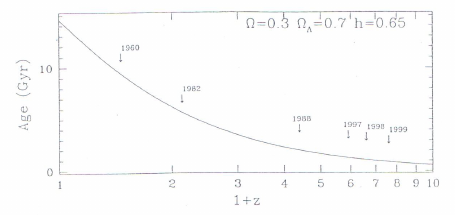
\includegraphics[width=0.85\textwidth]{Img/bertin_6.png}
\end{figure}

Nel grafico riportato in figura è segnata l'età dei corpi celesti ($Gyr$ indica $10^9$ anni) in funzione del redshift; le frecce con associate gli anni rappresentano gli oggetti più distanti di cui fosse nota la distanza (e la natura) nei periodi segnati. Il valore di redshift di un oggetto, come abbiamo già visto, è dato dal rapporto fra $\Delta \lambda=\lambda_o-\lambda_e$ e $\lambda_e$ e, per basse velocità, è circa il rapporto fra la velocità dell'oggetto e la velocità della luce ($z \ll 1$); dunque, per oggetti di recente formazione abbiamo che  il valore di redshift è più alto, poichè la velocità a cui viaggiano è ancora molto elevata. Questo concetto è ben spiegato dalla \textbf{legge di espansione di Hubble}, secondo la quale si ha che la velocità dell'oggetto è direttamente proporzionale alla sua distanza dalla Via Lattea (posta come centro di osservazione):
$$v=H_0 D \text{   con } H_0 \sim 70 \frac{km/s}{Mpc}$$
se il grafico fosse aggiornato alle nostre conoscenze attuali, avremmo che l'intercetta sarebbe a $13,6$ (miliardi di anni) mentre l'oggetto più distante sarebbe al valore di redshift $z=11$ per un età di circa $10^9$ (un miliardo) anni. Le varie costanti del tipo ``$\Omega$'' rappresentano dei parametri cosmologici, mentre $h$ è la variante adimensionale di $H_0$.
\vspace{0.05cm}
\\
\begin{minipage}{.60\textwidth}
	Nel grafico a destra, invece, abbiamo la dimensione angolare (cioè l'angolo sotteso) di un oggetto celeste in funzione del suo valore di redshift. Per tutte le curve traccaite il minimo si trova fra $z=1$ e $z=2$ e corrisponde ad una dimensione angolare di qualche secondo d'arco; la stranezza è che, dopo questo valore, la dimensione angolare ricomincia ad aumentare, cosa che ci indicherebbe che più un oggetto è distante, più ``il cielo è grande'', cioè l'angolo sotteso è maggiore.
\end{minipage}
\begin{minipage}{.40\textwidth}
	\centering
	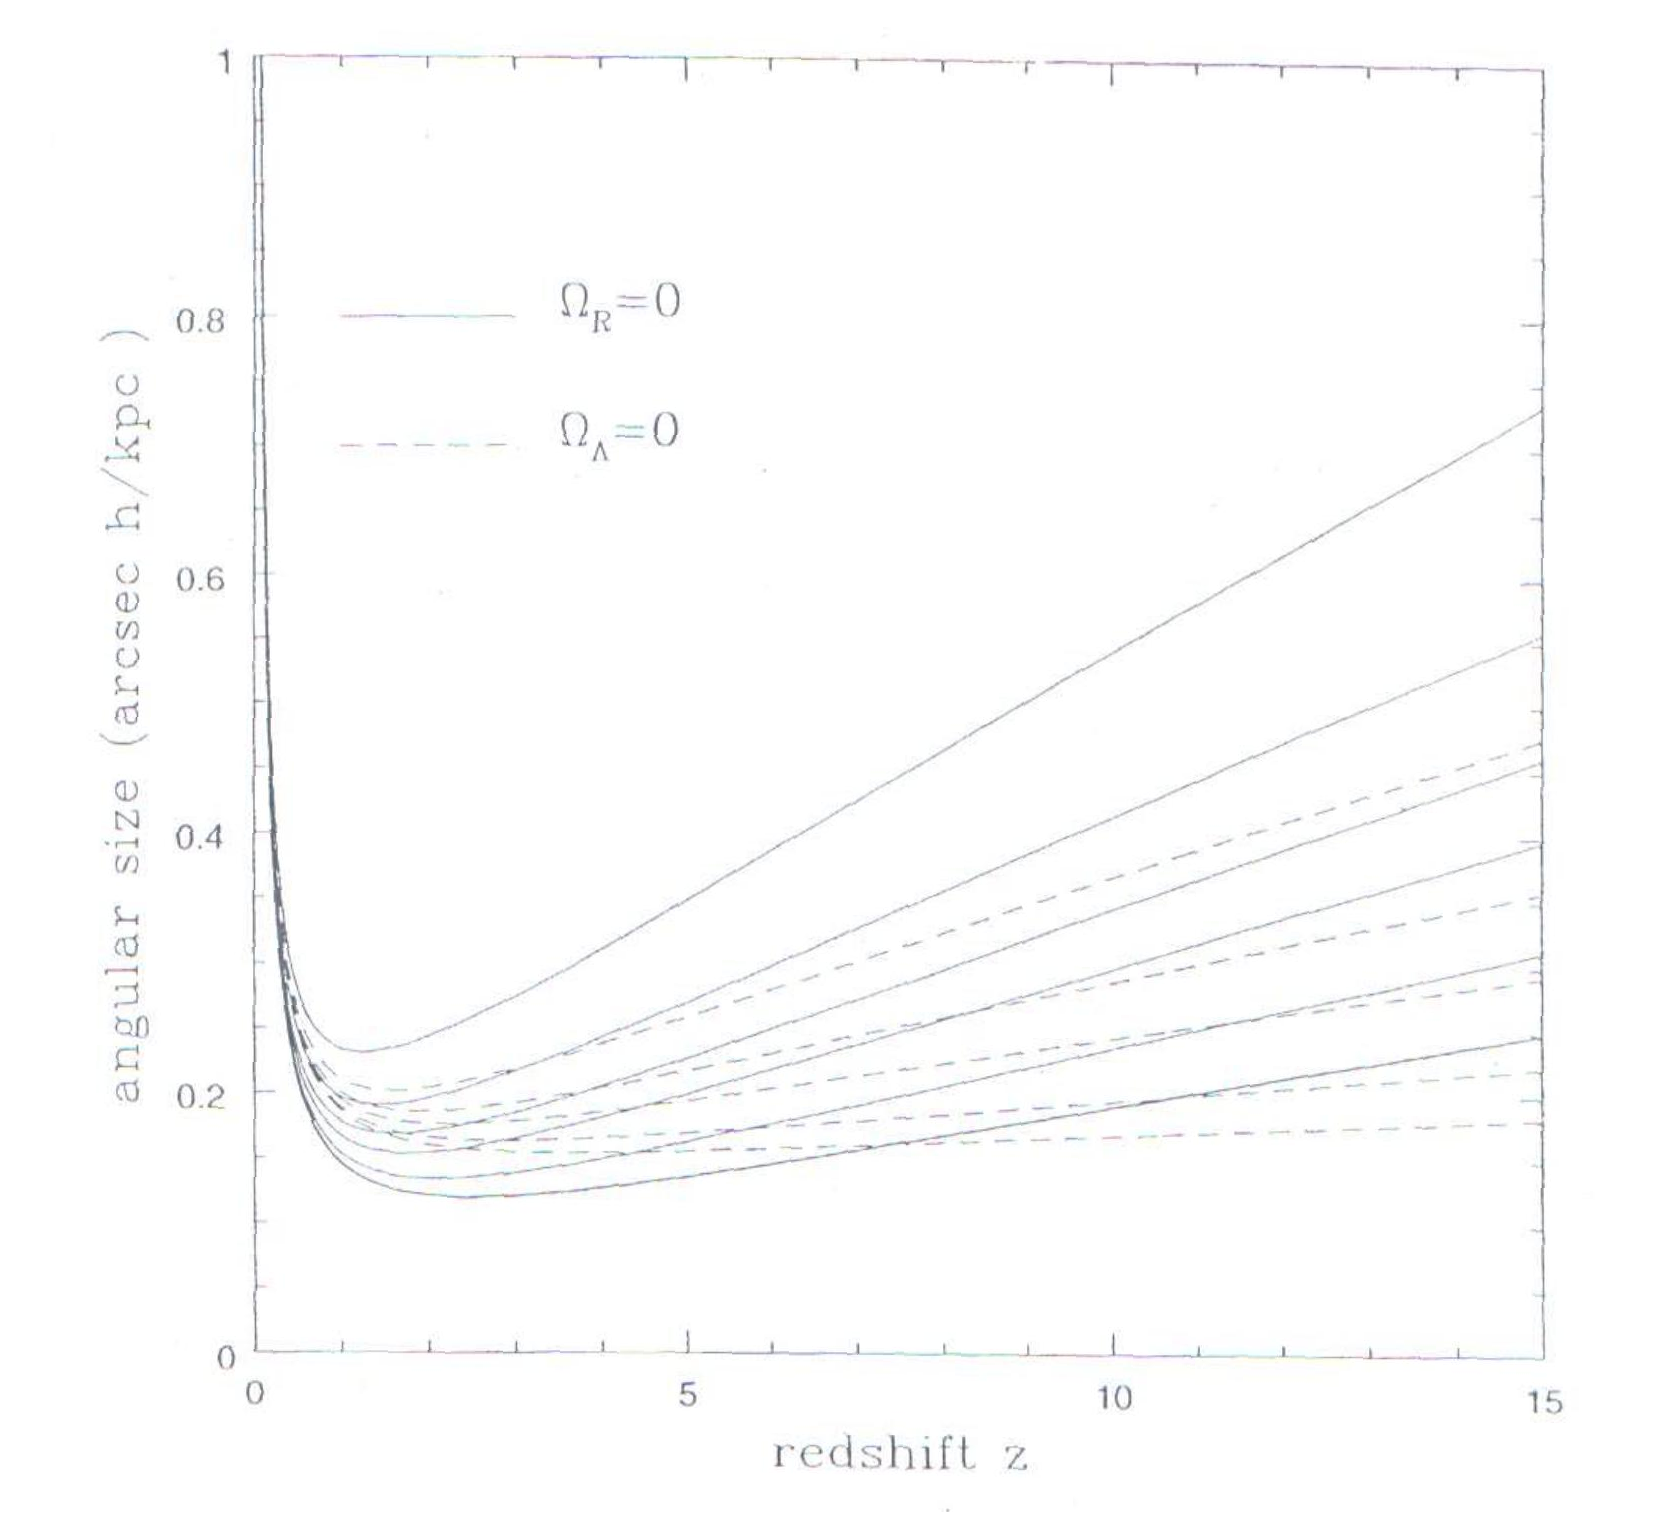
\includegraphics[width=1\textwidth]{Img/bertin_6bis.png}
\end{minipage}

\subsection{Moti radiali e moti propri}
Nell'introdurre il fenomeno di redshift abbiamo detto che esso è legato all'effetto doppler, e dunque da esso possiamo ricavare la velocità della stella; bisogna però stare attenti, poichè tale velocità risulta in realtà essere solo la componente ``radiale'', cioè la componente nella direzione dell'osservazione: chiameremo questa velocità $v_r$ (dove la $r$ sta per radiale) o $v_{los}$ (dove $los$ sta per line of sight).
\\
Consideriamo il solito cluster $\omega$-Centauri: possiamo misurare la velocità radiale per ogni stella, ottenendo una famiglia di velocità
$$\left\{ v_{los} ^{(n)} \right\}_{n=1} ^N$$
dove $N$ è il numero totale di stelle; di questa famiglia possiamo poi effettuare una media, ottenendo il valore $\langle v_{los} \rangle$  che mi descrive con buona approssimazione come l'oggetto completo si muove; possiamo infatti prendere questo valore come rappresentativo della velocità del baricento (in teoria dovremmo conoscere tutte le masse, ma esse risulterebbero molto simili fra loro e dunque si otterrebbe un risultato simile a $\langle v_{los} \rangle$). Possiamo inoltre considerarne lo scarto quadratico medio: $$\sqrt{\langle \left(v_{los}^{(n)}- \langle v_{los} \rangle \right)^2 \rangle}$$
che chiameremo \textbf{dispersione di velocità}; nel caso di $\omega$-Centauri, si ha una dispersione di velocità tipica di circa $5 \, \frac{km}{s}$, che risulta essere molto bassa (da un punto di vista astronomico: abbiamo infatti che la velocità con cui la Terra ruota intorno al Sole è di circa $30 \, \frac{km}{s}$, mentre la velocità con cui il Sole ruota intorno al centro della Via Lattea è di circa $200 \, \frac{km}{s}$).

Possiamo ricavare anche la componente ortogonale della velocità misurando lo spostamento angolare in un anno (si parla in questo caso di \textbf{moti propri}); l'unità di misura è quindi in secondi d'arco per anno $\left(\frac{''}{yr}\right)$. Prendendo ancora come esempio $\omega$-Centauri, è stato misurato un valore pari a $10^{-3} \, \frac{''}{yr}$.\\
Per convertire la misura nel canonico $\frac{km}{s}$, dobbiamo conoscere il valore della distanza dall'oggetto osservato (vale infatti che $v=\omega D$), ma ricavare questo valore è spesso difficile; per ovviare a questo problema si sfruttano i risultati di Poincarè, secondo cui, come avevamo già accennato all'inizio, un ammasso stellare è affine ad un gas all'equilibrio termodinamico. Possiamo dunque utilizzare la \textbf{distribuzione di Maxwell-Boltzmann}:
$$f=A e^{-\frac{E}{kT}}$$
dove $E$ è la'energia cinetica, mentre $k$ è la costante di Boltmann; utilizzando questo espediente siamo in grado di calcolare $D$, e dunque ci togliamo dall'impiccio di non conoscere la distanza dall'ammasso stellare.\\
Il problema si basa sullo scarto quadratico medio; scriviamo:
$$f=A e^{-\frac{E}{kT}}=A e^{-\frac{m}{2kT} v^2}= A e^{-\frac{v^2}{2 v_{th} ^2}} = A e^{-\frac{v_{los} ^2 + v_{\perp} ^2}{2 v_{th} ^2}}$$
dove abbiamo definito la \textbf{velocità termica} $v_{th}=\sqrt{\frac{kT}{m}}$, che risulta essere una costante; in termini matematici, la velocità termica è la dispersione della gaussiana associata alla distribuzione. Il fatto che si instauri una situazione modellizzabile tramite la distribuzione di Maxwell-Boltzmann ci dice che la dispersione dei moti lungo  la linea di vista deve essere uguale a  quella lungo la sua direzione ortogonale; imponendo questa condizione possiamo misurare $v_{\perp}$, e dunque ricavare la distanza $D$. In questo modo otteniamo una misura dinamica della distanza $D$.

\subsection{Popolazioni stellari}
Il concetto di popolazione stellare è idealmente abbastanza semplice: infatti chiamiamo in questo modo un insieme di stelle che, per forza di cose, non sono tutte uguali (per fissare meglio il concetto, possiamo prendere come esempio l'aria che è composta da diversi atomi; allo stesso modo, tali insiemi di stelle sono composte da stelle di tipo e dimensioni diverse). Ogni stella contribuisce all'emissione in maniera diversa; ma, fintanto che la popolazione stellare ha caratteristiche fisse, si ha che i valori di massa e luminosità rimangono costanti. Il concetto appena espresso si può capire prendendo ad esempio la Via Lattea: infatti, prendendo della sferette di raggio $100 \, pc$ nella zona in cui si trova il sistema solare, abbiamo che le ``composizioni stellari'' di tali sferette (cioè le stelle che appartengono a questi insiemi) sono molto simili, e dunque i loro valori di massa e luminosità si assomigliano; questo ci fa capire che esiste un rapporto di proporzionalità fra la massa $M$ e la luminosità $L$.

\section{Radio astronomia}
Se volessimo andare indietro per vedere quando i fisici e gli astrofisici hanno cominciato a misurare nella banda delle onde radio, arriveremmo più o meno intorno agli anni '30, con delle prime misurazioni abbastanza ``primitive''; risale a quel periodo il lavoro sulle onde radio dell'astronomo americano Jamsky, da cui poi prende il nome l'unità di misura tipica delle onde radio.\\
La vera svolta arriva nel 1965, anno in cui Penzias e Wilson scoprirono il cosìddetto \textbf{fondo cosmico di microonde} (CMBR, Cosmic Microwave Background Radiation), cioè la luce del Big Bang così come la vediamo noi $13,5$ miliardi di anni dopo; i due astronomi, puntando le loro antenne verso il cielo, si accorsero che stavano misurando un segnale e, ripulendo via via il segnale da tutte le possibili fonti di onde radio, arrivarono a scoprire un fondo di segnale fisso, che poi venne identificato con la radiazione del Big Bang. In particolare, una cosa che ebbe e ha tutt'ora un impatto enorme è la \textbf{radiazione a $21 \, cm$}; che, se andiamo a controllare la tabella con le varie lunghezze d'onda, corrisponde ad una frequenza di circa $1420 \, MHz$; quando parliamo di $21 \, cm$ ci stiamo riferendo ad una riga di uno spettro, e nel nostro caso il responsabile di tale riga è l'idrogeno atomico (comunemente chiamato $H \RNum{1}$)\footnote{La nomenclatura per l'idrogeno nelle varie forme in cui si presenta in natura è $H \RNum{1}$ (si legge H uno) per l'idrogeno atomico, $H_2$ per l'idrogeno molecolare e $H \RNum{2}$ (H due) per l'idrogeno ionizzato; per quest'ultimo, si sente spesso parlare di ``regioni $H \RNum{2}$'', cioè di zone in cui è presente in gran quantità l'idrogeno ionizzato (ad esempio, nella nebulosa di Orione).}.\\
Tale radiazione venne scoperta a tavolino per merito di uno studente al quale venne commissionato come tesi di dottorato il compito di trovare una riga nelle onde radio, cioè di trovare una transizione che cadesse in tale fascia; sin da subito tale riga venne associata allo spettro dell'idrogeno, ma bisognerà aspettare il 1951 per avere una sua misuraspecifica (ad opera di Ewen e Purcell).\\
Nel 1958 Oort, Kerr e Westerbout, sfruttando la scoperta della radiazione a $21 \, cm$, scrissero un articolo da cui è tratta l'immagine a lato; in tale immagine è indicata la distribuzione di idrogeno nel piano della galassia in una scala di densità di $\frac{\# \, atomi}{cm^3}$; le informazioni che possiamo ricavare da questa immagine sono:\\
\vspace{0.05cm}\\
\begin{minipage}{.65\textwidth}
\begin{itemize}
	\item Nella Via Lattea c'è tantissimo idrogeno
	\item Le zone colorate in grigio-nero rappresentano la posizione del segnale di cui è stata misurata posizione e densità
	\item Ci sono due coni vuoti, cioè due zone in cui non è stato misurato nulla; queste sono dovute al metodo di misura utilizzato, che risulta essere inutilizzabile puntando il centro della galassia o i suoi antipodi.
\end{itemize}
\end{minipage}
\begin{minipage}{.35\textwidth}
	\centering
	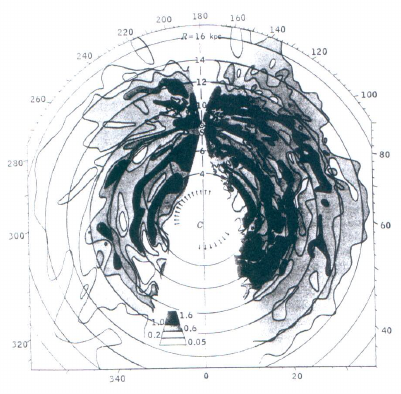
\includegraphics[width=1\textwidth]{Img/bertin_7.png}
\end{minipage}
\vspace{0.05cm}\\
Questa immagine è spesso indicata come prima evidenza del fatto che la nostra galassia abbia la forma di una spirale; la seconda immagine che riportiamo rappresenta una curva di rotazione del gas, cioè a che velocità esso ruoti rispetto al centro della galassia (in funzione della riga a $21 \, cm$).

\begin{figure}[h!]
	\centering
	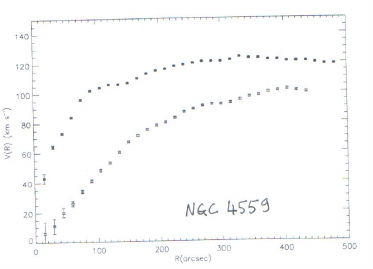
\includegraphics[width=0.5\textwidth]{Img/bertin_7bis.png}
\end{figure}

\section{Pulsar}

\begin{figure}[h!]
	\centering
	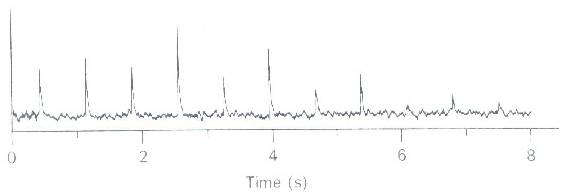
\includegraphics[width=1\textwidth]{Img/bertin_8.png}
\end{figure}

Le pulsar sono particolari tipi di stelle che emettono un segnale molto regolare della forma di quello riportato qua sopra; tale segnale presenta sia dei picchi (temporalmente) equidistanti sia delle irregolarità ma, attraverso un analisi temporale, è possibile estrarre una frequenza molto pulita, segno che tali irregolarità, sono limitate alla sola forma del segnale. In particolare, il segnale nel grafico ha un periodo di $0,714 \, s$, ma sono state osservate pulsar con periodo nell'ordine dei $ms$; questo limite è dovuto ai metodi di misura, che non permettono di raggiungere una precisione maggiore e dunque di distinguere eventuali pulsar con periodi più bassi.
\\

In realtà è errato parlare di pulsar, poiché si fa riferimento al concetto di pulsazione che in questo caso non è appropriato: infatti dire che un oggetto sta pulsando equivale a dire che tale oggetto si sta ciclicamente gonfiando e sgonfiando; in questo caso la pulsazione non è dovuta ad un processo di dilatazione e contrazione\footnote{Un ciclo dilatazione-contrazione è osservabile nelle Cefeidi (\url{https://it.wikipedia.org/wiki/Variabile_Cefeide}), stelle che con un periodo nell'ordine di qualche giorno si dilatano e si contraggono.} ma ad una rotazione, e l'evidenza di questo fatto è proprio la precisione temporale con cui il segnale si ripresenta, cioè il fatto che sia possibile estrarre in maniera molto precisa un periodo (di rotazione).\\
Le pulsar sono spesso legate all'esplosione di una supernova, e dunque si trovano nella maggior parte dei casi all'interno di nebulose; una nebulosa, detta anche \textbf{supernova remnant}, è una regione di cielo in cui rimangono i residui dell'esplosione di una supernova, come ad esempio la nebulosa del Granchio (M1), formatasi a seguito dell'esplosione di una supernova osservata sulla Terra nel 1054. Nel caso delle supernove l'esplosione è associata ad un implosione della stella, cioè avvengono contemporaneamente un rilascio di materia stellare e un collasso della stella stessa; da tali implosioni possono facilmente generarsi delle pulsar, cioè degli oggetti molto compatti che spesso sono identificati con le \textbf{stelle di neutroni}. Questi oggetti hanno una massa molto simile a quella del Sole ($M_{NS} \sim M_{odot}=2 \cdot 10^30 \, kg$) ma, mentre quest'ultimo ha raggio $R_{\odot}= 7 \cdot 10^5 \, km$, il raggio di una stella di neutroni è nell'ordine di qualche $km$\footnote{Per oggetti nell'ordine di una $M_{\odot}$ il raggio di Schwarzschild, cioè il raggio entro cui è definito l'orizzonte degli eventi (oltre le quali si forma un buco nero, si veda \url{https://it.wikipedia.org/wiki/Raggio_di_Schwarzschild} per maggiori informazioni), è di circa $3 \, km$.}; un'altro oggetto molto compatto è la nana bianca, anch'essa avente massa $M_{WD} \sim M_{\odot}$ ma con raggio $R_{WD} \sim 10^4 \, km$ (circa come il raggio terrestre).

\clearpage

\begin{tikzpicture}[remember picture,overlay] 
\pgfdeclareimage[width=\paperwidth]{image}{Img/bertin_9.jpg}
\node at (current page.center) {\pgfuseimage{image}}; 
\end{tikzpicture}

\clearpage

\subsubsection{Note alla scheda:}
In questa scheda sono contenute informazioni riguardo alcune pulsar.\\
Le pulsar presenti nella nebulosa del Granchio, nonostante abbiano un periodo di rotazione nell'ordine di un secondo, sono state considerate per molti anni le pulsar più veloci, fino alla scoperta delle millisecond pulsar; queste ultime sono pulsar con periodi di rotazione nell'ordine di $1 \, ms$, e hanno la particolarità di essere state sempre osservate all'interno dei cluster stellari.\\
Una parola ricorrente è il termine \textbf{glitches}: traducibile con ``scossoni'' o ``terremoti'', si tratta di modifiche (diminuzioni) del periodo di rotazione causate da assestamenti e modifiche della forma fisica della stella\footnote{Per saperne di più, vedere \url{https://it.wikipedia.org/wiki/Glitch_(astronomia)}.}.\\
Infine, degna di nota è la scoperta nel 1974 dell'oggetto denominato Hulse-Taylor binary, che è la prima pulsar binaria scoperta.
%non bellissima questa parte...
\\
\\
Il prossimo passo è provare a dimostrare che se le pulsar sono delle stelle di neutroni allora devono per forza essere dei ``rotatori'', cioè la pulsazione è dovuta ad una rotazione; per fare ciò, sfruttiamo le millisecond pulsar e approssimiamo la superficie del nostro oggetto ad una sfera.\\
Immaginiamo di avere una massa piccola ($m \ll M_{NS}$) posata sulla superficie della stella all'altezza dell'equatore: che condizioni si devono verificare perchè tale massa si trovi in equilibrio così come noi siamo in equilibrio sulla Terra? Si deve avere che $F_{grav}>F_{centr}$; notiamo che non usiamo ``$\geq$'', poichè altrimenti se si verificasse la condizione di uguaglianza avremmo che l'oggetto entrerebbe in orbita. La disuguaglianza fra forze si traduce in:
$$m a_g > m \Omega^2 R \implies a_g > \Omega^2 R$$
dove $R$ è il raggio della stella, $\Omega= \frac{2 \pi}{T}$ è la frequenza a cui ruota e $m$ la massa presa in considerazione; notiamo che la massa gravitazionale e la massa inerziale (rispettivamente a sinistra e a destra del segno di disuguaglianza) si cancellano, segno che il valore della massa è irrilevante nel nostro studio (purchè si abbia $m \ll M_{NS}$, in modo tale che non ci siano effetti macroscopici dovuti alla gravità). Dalla legge di gravitazione universale ricaviamo che $a_g=\frac{GM_{NS}}{R^2}$; inoltre non stiamo facendo nessuna ipotesi sull'omogeneità della massa, e dunque avremo $M_{NS}= \int_0 ^R \rho(r) 4 \pi r^2 dr$; dato che deve valere la simmetria sferica, possiamo definire una densità media:
$$\langle \rho \rangle=\frac{M_{NS}}{\frac{4}{3} \pi R^2}$$
Sostituendo all'interno della disuguaglianza quanto appena trovato, si ottiene:
$$\frac{GM_{NS}}{R^2}>\Omega^2 R \implies \frac{GM_{NS}}{\frac{4}{3} \pi R^2}>\Omega^2 R \frac{1}{\frac{4}{3} \pi} \implies \frac{GM_{NS}}{\frac{4}{3} \pi R^3}> \frac{3 \Omega^2}{4 \pi} \implies$$
$$\implies G \langle \rho \rangle > \frac{3 \Omega^2}{4 \pi}= \frac{4 \pi^2}{T^2} \frac{3}{4 \pi} \sim \frac{10}{T^2}$$
A questo punto, invertendo la relazione e sostituendo i valori di $G$ e $T$, otteniamo
$$\langle \rho \rangle \gtrsim \frac{10}{G T^2} \sim 10^ {15} \frac{g}{cm^3}$$
che è il valore tipico della densità nucleare; dunque è lecito ipotizzare che le pulsar siano effettivamente stelle a neutroni.

\subsection{Pulsar binarie}
Abbiamo già citato la Hulse-Taylor binary in quanto prima pulsar binaria scoperta; con questo termine ci si riferisce ad una pulsar che fa parte di un sistema binario in cui la seconda stella è un oggetto compatto (nana bianca, stella a neutroni...) ma non è detto che sia anch'essa una pulsar.\\
Nel caso della Hulse-Taylor siamo in presenza di due stelle di neutroni: il periodo della pulsar è di $59 \, ms$, il periodo orbitale della binaria è $7$ ore e $45$ minuti e la distanza fra le due stelle è circa $700000 \, km$; la sua scoperta fruttò il premio nobel a Hulse e Taylor. Di tale sistema binario si è notato che il periastro, cioè la distanza minima a cui si avvicinano le due stelle, è di circa un $R_{\odot}$ e che periodo orbitale col passare del tempo va diminuendo, cioè le due stelle ruotano sempre più velocemente; tale variazione è pari a $\Delta \dot{R} \sim 1 \, \frac{cm}{giorno}$ ($R$ indica il periastro), e rimanda al fatto che el due stelle stanno cadendo una sull'altra per effetto della perdita di energia tramite l'emissione delle onde gravitazionali; questa tesi è supportata dal fatto che i dati in nostro possesso siano quasi perfettamente in accordo con la predizione teorica. Dunque grazie alla pulsar di Hulse-Taylor abbiamo avuto una prima evidenza dell'esistenza delle onde gravitazionali.
%voice00029 min 40

\section{Lenti gravitazionali}
\begin{minipage}{.40\textwidth}
	\centering
	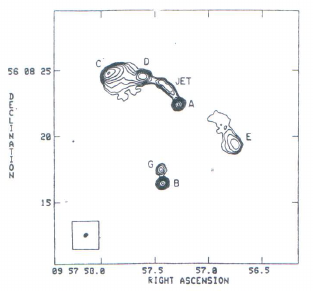
\includegraphics[width=1\textwidth]{Img/bertin_11.png}
	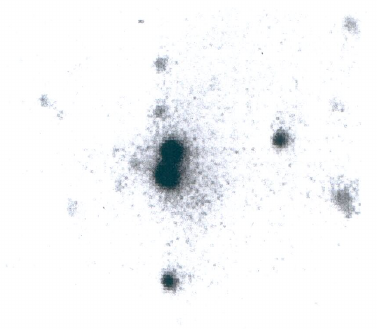
\includegraphics[width=1\textwidth]{Img/bertin_11bis.png}
\end{minipage}
\begin{minipage}{.60\textwidth}
	Nelle due immagini a lato possiamo vedere lo stesso pezzo di cielo osservato attraverso un radiotelescopio (in alto) e un telescopio ottico (in basso); in particolare, ci soffermiamo sugli oggetti che nella prima immagine sono etichettati con le lettere A e B: sappiamo che si tratta di quasar\footnote{Le quasar (QUASi-stellAR objects) sono oggetti nel cielo molto luminosi e generalmente molto distanti dalla Terra; per maggiori informazioni, vedere \url{https://it.wikipedia.org/wiki/Quasar}.}, ma la domanda che ci si pone è se i rispettivi segnali siano relativi a due sorgenti diverse o alla stessa sorgente. La risposta a tale domanda può suonare strana, ma i due oggetti in questione sono effettivamente l'immagine doppia di una stessa quasar; tali immagini sono una delle prime evidenze che portarono alla scoperta delle lenti gravitazionali.
\end{minipage}
Questo fenomeno è spesso dovuto alla presenza di una galassia, detta galassia-lente, che modifica l'immagine dell'oggetto osservato (che si troverà ``dietro'' di essa) deformandola o facendone apparire la figura in più punti nei suoi dintorni. Nel caso particolare riportato qua sopra, abbiamo una galassia-lente a redshift $z \sim 0,36$ a metà fra le due immagini A e B che hanno invece $z \sim 1,4$; l'analisi spettroscopica di tali oggetti ci permette di concludere che si tratta effettivamente dell'immagine sdoppiata della stessa quasar.

Un caso particolarmente importante  di lente gravitazionale è quello legato alla nebulosa Refsdal ($z=1,49$), la cui immagine venne riprodotta in quattro punti diversi intorno all'ammasso di galassie MACS J1149.6+2223 ($z=0,544$) a formare una croce detta croce di Einstein.\footnote{Ci rifacciamo all'articolo \url{http://www.nature.com/news/supernova-kaleidoscope-seen-for-first-time-1.17062}, dal quale è anche stata presa la foto.}

\begin{figure}[h!]
	\centering
	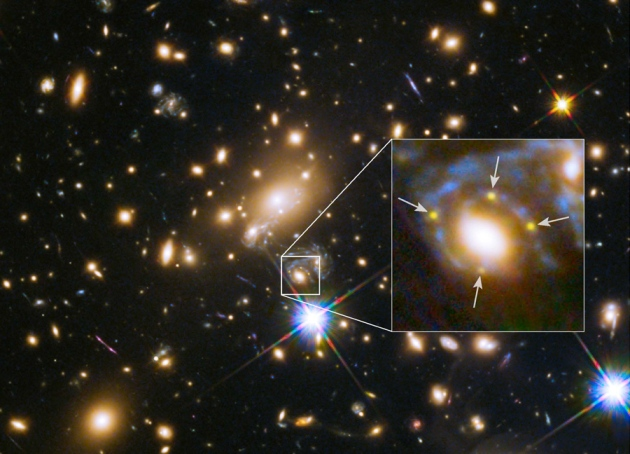
\includegraphics[width=0.6\textwidth]{Img/lente_grav.jpg}
\end{figure}
Tali immagini però ``apparvero'' nel cielo in tempi differenti; gli astronomi, partendo dalla prima apparizione, riuscirono a calcolare in maniera abbastanza precisa quando sarebbero apparse le altre tre immagini, verificando poi che i loro calcoli erano esatti; dunque le osservazioni legate a questa supernova rappresentano un notevole passo avanti nello studio del fenomeno delle lenti gravitazionali.

\section{Astrofisica X}
La storia dell'astrofisica X, cioè dello studio dell'universo nella regione dei raggi X, ha inizio negli anni '60, in piena guerra fredda; in quel periodo, infatti, gli astronomi americani si accorsero che mandando in orbita un satellite era possibile compiere osservazioni in bande che erano schermate dall'atmosfera, e che dunque non erano osservabili da terra. Fra i primi ad avere questa intuizione ci fu un astronomo italiano che viveva in America, Bruno Rossi, il quale riuscì a convincere\footnote{Per convincerli pose come obbiettivo primario della missione il verificare se la luna fosse o meno sorgente di raggi X (che sarebbero stati dannosi per gli astronauti); una volta completato tale obbiettivo e verificato che la Luna non era ``pericolosa'', il telescopio venne puntato altrove e iniziò a raccogliere segnali esterni.} il governo americano a dare i fondi per mandare un telescopio X nello spazio; grazie a tale strumento, fu possibile scoprire che le fonti di tali radiazioni X erano dei particolari oggetti celesti, le \textbf{binarie X}.\\
Tali oggetti sono un sistema binario formato da due stelle molto diverse tra loro: abbiamo infatti un oggetto spazialmente piccolo ma più massivo (stella di neutroni, nana bianca, buco nero) e una stella che spazialmente è più grande ma la massa è meno concentrata rispetto alla stella a neutroni; la struttura di questo sistema non è da immaginare come due stelle che ruotano intorno al loro centro di massa, ma a causa della mutua forza di gravità ($F_{g}^{S1} \gg G_{g}^{S2}$) assume una forma più ``irregolare'' detta \textbf{lobo di Roche}. Oltretutto, in tali sistemi si osserva che la stella meno massiva ``cade'' nell'oggetto più massivo, generando intorno a quest'ultima delle nubi di gas dette \textbf{dischi di accrescimento}; il sistema viene detto binaria X poichè l'oggetto più massivo, nel processo di assorbimento dei gas esterni dell'altra stella, presenta salti di energia che causano l'emissione di radiazione X.

\vspace{0,15cm}
\begin{minipage}{.45\textwidth}
	\centering
	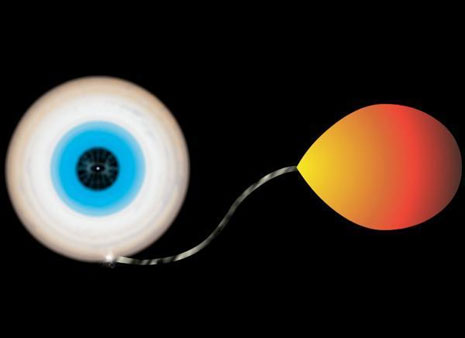
\includegraphics[width=0.875\textwidth]{Img/lobo_roche.jpg}
\end{minipage}
\begin{minipage}{.45\textwidth}
	\centering
	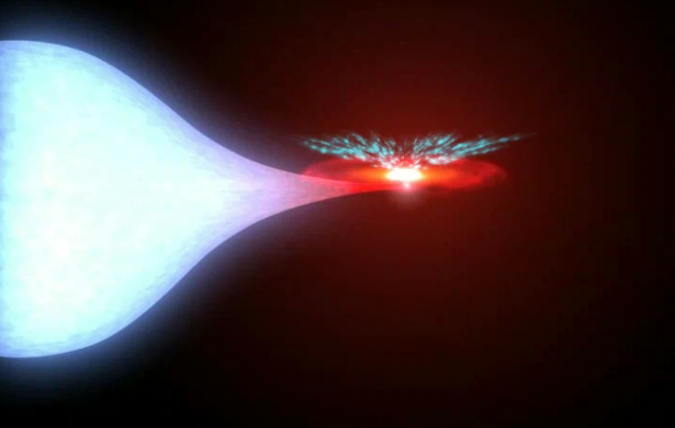
\includegraphics[width=1\textwidth]{Img/binaria_x.png}
\end{minipage}

\vspace{0,15cm}

Il modello dei dischi di accrescimento e dell'emissione di raggi X ebbero parecchio successo in ambito astrofisico, tanto che allla scoperta delle quasar si è ipotizzato che la fenomenologia fosse molto simile; questo nonostante le binarie X siano astronomicamente giovani (la prima scoperta è datata 1962).
\\
Un enorme passo avanti nello studio dell'universo dal punto di vista della radiazione X è stato fatto negli anni '70, durante i quali quella che era un'astronomia rudimentale venne portata ad un livello di ottica capace di ottenere delle immagini degli oggetti osservati (imaging).
\\

Esistono degli oggetti molto grandi che possono essere indicati come ammassi di galassie; il più vicino a noi è il Virgo cluster of galaxyes (ammasso di galassie della Vergine), rispetto al quale noi siamo quasi in periferia (infatti i moti nella Via Lattea risentono di deviazioni dovute alla forza di gravità che esercita tale ammasso di galassie); per dare un'idea delle dimensioni, è composto da circa 2000 galassie distribuite nel cielo in circa 20 gradi; l'ammasso ha dimensioni di $1 \, Mpc$ e si trovano ad una distanza dalla Terra di $15 \, Mpc$.\\
La scoperta di molti di questi oggetti è attribuita a due astronomi statunitensi, Zwicky e Abell; con l'avvento dell'astronomia X venne inoltre scoperto che le galassie nei cluster non sono nel vuoto ma sono immerse in un ``mare'' di radiazione X che loro stesse producono; tale mezzo intergalattico (\textbf{ICM, IntraCluster Medium}) è prodotto tramite un processo detto bremmstrahlung (traducibile come ``radiazione di frenamento'') che indica il processo mediante il quale una particella, urtando contro un elettrone atomico, perde energia cinetica sotto forma di fotone X. Le temperature del ICM sono circa $5-10 \, KeV$ (corrispondenti a circa $60-120 \cdot 10^3 \, K$), e dunque data la temperatura siamo in presenza di plasma; nel grafico  riportato qua sotto possiamo vedere le temperature di alcuni ammassi in funzione del loro raggio.

\begin{figure}[h!]
	\centering
	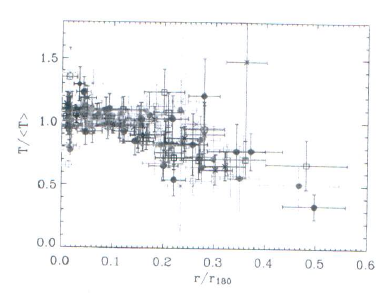
\includegraphics[width=0.35\textwidth]{Img/bertin_12.png}
\end{figure}

\section{Astronomia $\gamma$}

\begin{figure}[h!]
	\centering
	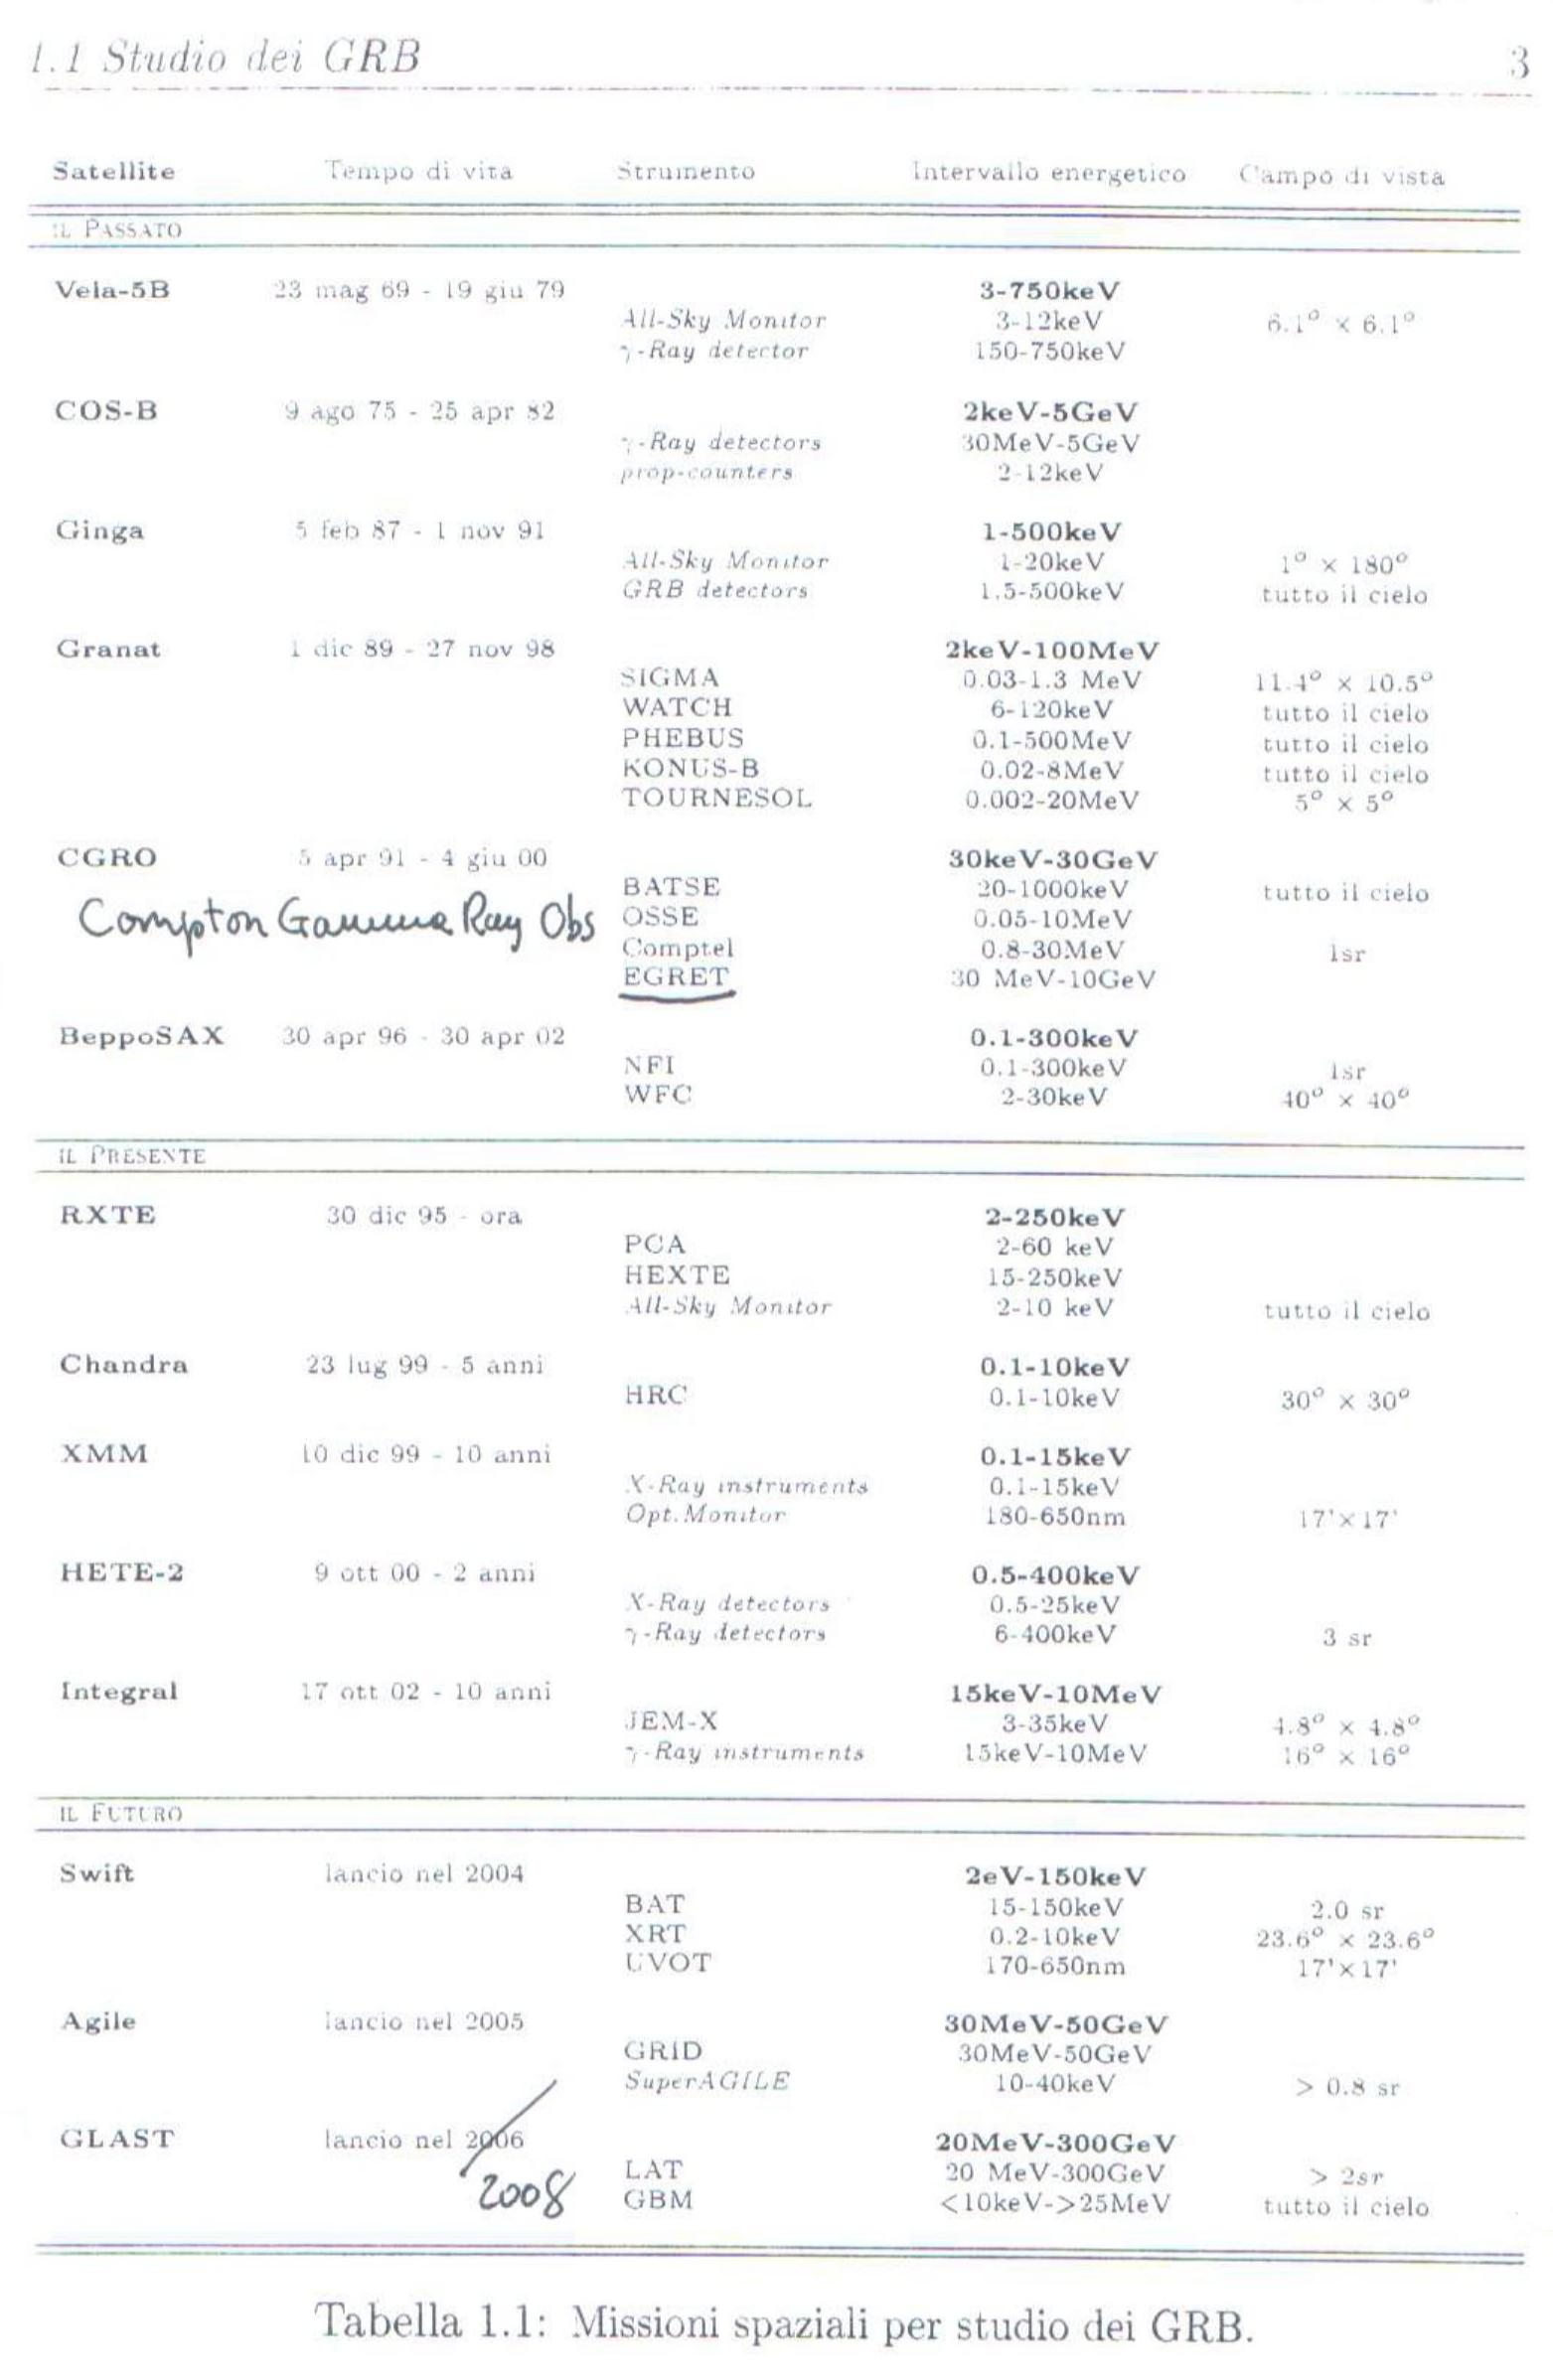
\includegraphics[width=0.8\textwidth]{Img/bertin_13.jpg}
\end{figure}

Nella tabella riportata sopra (tratta da una tesi di laurea del 2004) sono riportate le principali missioni passate o tutt'ora attive legate allo studio dei \textbf{GRB}, \textbf{Gamma Ray Burst} ; questi fenomeni consistono nell'emissione di massicce quantità di raggi gamma da parte di buchi neri in accrescimento.\\
La scoperta dei GRB avvenne ``per caso'' nel 1967 tramite il satellite Vela: infatti lo scopo della missione americana era quello di rivelare i raggi gamma provenienti da eventuali esplosioni di bombe atomiche russe, in modo tale da smascherare gli esperimenti dei rivali (siamo in piena guerra fredda); ma la quantità di raggi gamma era talmente alta da portare gli scienziati ad escludere che essi fossero dovuti a esplosioni di bombe sovietiche. Si dovrà però aspettare il 1997, con la missione italo-olandese Beppo-SAX, per identificarne la provenienza: infatti il satellite aveva a bordo una batteria di telescopi diversi, che permettevano osservazioni di radiazione $\gamma$, X e ottica\footnote{Il motivo per cui vennero utilizzati telescopi diversi è diversa precisione con cui i vari strumenti posso dare l'indicazione di provenienza: mentre i telescopi $\gamma$ danno una pessima indicazione di provenienza, abbiamo che i telescopi ottici sono i migliori da questo punto di vista.}; non appena i telescopi $\gamma$ acquisivano uno di questi GRB, i telescopi X e ottici si attivavano e iniziavano ad osservare nella direzione da cui provenivano i $\gamma$, coadiuvati da telescopi da Terra. In questo modo, si scoprì che i GRB sono fenomeni extra-galattici che hanno luogo in galassie molto lontane e deboli. La sua eredità è passata a Swift, che evolve l'idea di base di Beppo-SAX e ha permesso di individuare centinaia di GRB.
\\
Nella tabella riportata di sotto vediamo i dati relativi ad alcuni GRB rivelati; la nomenclatura di tali fenomeni è una sigla alfanumerica, dove alla sigla GRB segue un codice di sei cifre che ci dice, nell'ordine, anno, mese e giorno in cui è stato rivelato il raggio $\gamma$.

\begin{figure}[h!]
	\centering
	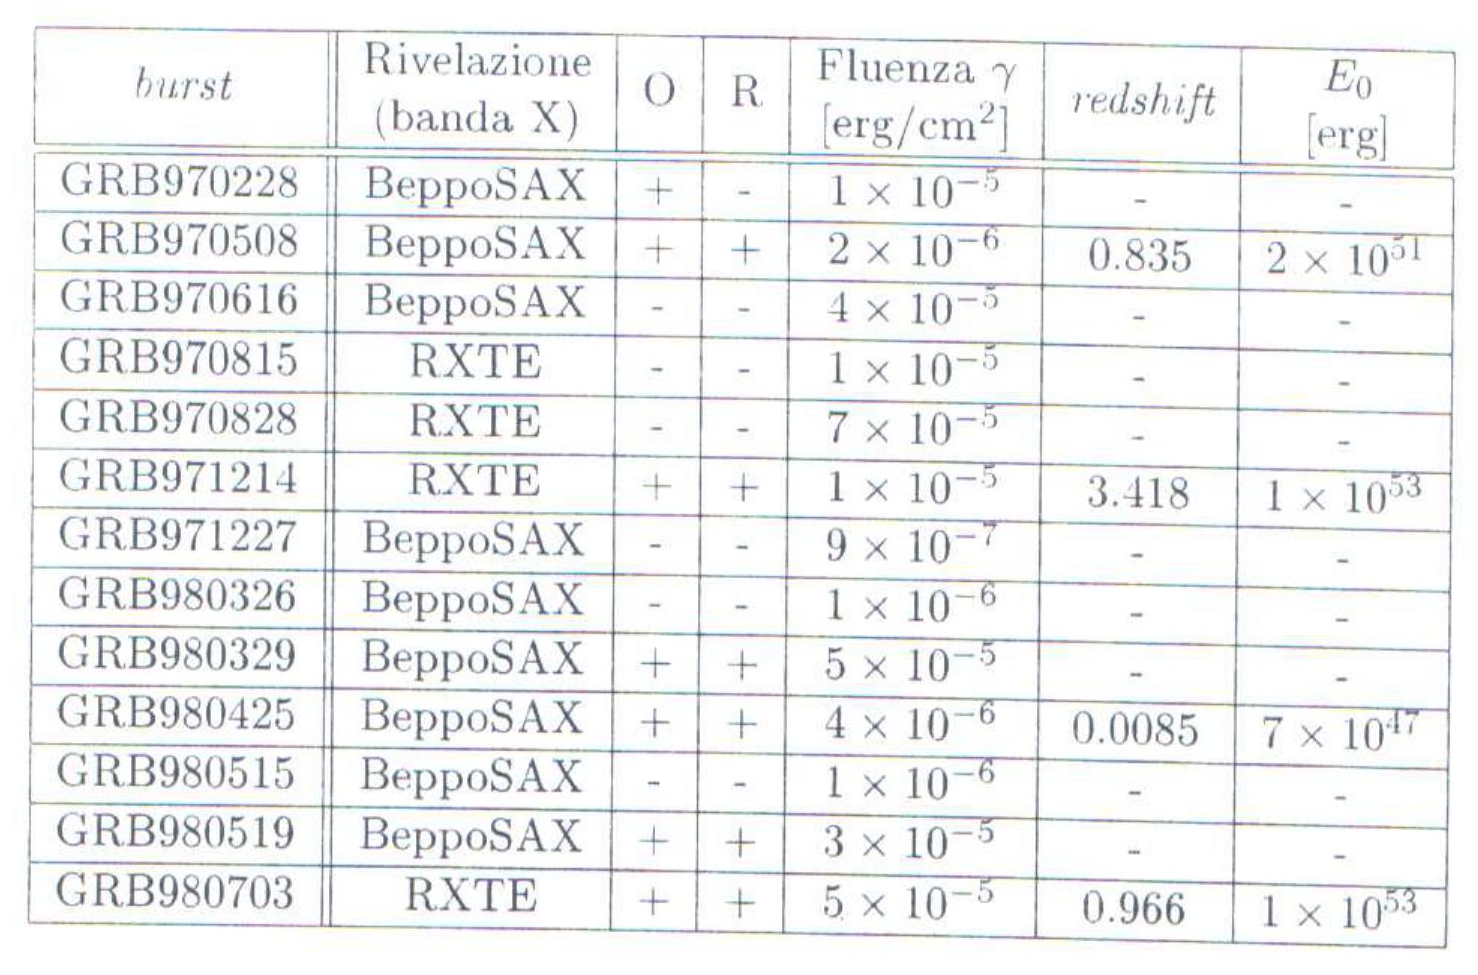
\includegraphics[width=0.8\textwidth]{Img/bertin_14.png}
\end{figure}

Grazie a queste osservazioni si è riuscito a capire che c'era in cielo una sorgente che era la causa di questo bagliore, che venne osservato anche nella regione dell'ottico (si parla di afterglow, cioè di un bagliore nell'ottico a seguito di un lampo gamma); si scoprì inoltre che tali sorgenti si trovavano all'interno di galassie, e per alcune di esse venne inoltre misurato il redshift. Una cosa curiosa è il fatto che i valori di redshift mosurati sono nell'ordine di  uno, segno che la fonte si trova a $7-8$ miliardi di anni luce; a questo punto, dal flusso osservato, possiamo ridurre la magnitudine e la potenza della sorgente e l'energia coinvolta nell'esplosione (alcuni dati sono riportati nella tabella di sopra).
\\
\begin{minipage}{.45\textwidth}
	\centering
	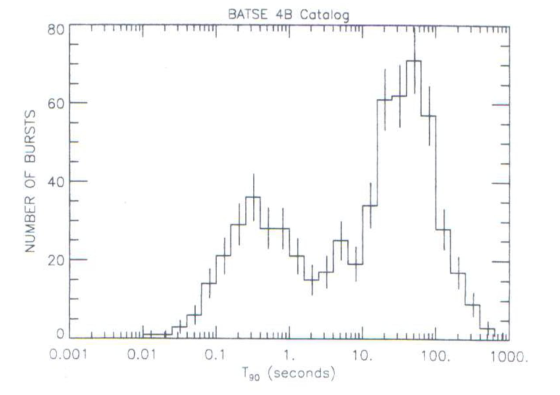
\includegraphics[width=0.875\textwidth]{Img/bertin_14bis.png}
\end{minipage}
\begin{minipage}{.50\textwidth}
Dai dati riportati nel grafico a lato possiamo notare come ci siano due tipi di GRB, che si differenziano a seconda della loro durata: quelli cosìddetti ``veloci'', che durano qualche secondo, e quelli ``lenti'' che invece durano qualche decina o centinaia di secondi.
\end{minipage}

Fra i meccanismi che agiscono e che permettono di osservare questi fenomeni c'è sicuramente l'esplosione di una supernova, e in effetti il bagliore ottico è spesso legato ad una supernova. Inoltre, sappiamo che tali fenomeni non sono direzionali, ma propagano in tutte le direzioni (angolo solido $4 \pi$): infatti se cosi non fosse osserveremmo dei fenomeni molto più potenti e soprattutto ne vedremmo molti meno (in media se ne osserva uno al giorno), poichè dovremmo avere la ``fortuna'' di essere nella direzione puntata dal GRB.
\\
Puntando i telescopi verso il centro della Via Lattea, si è scoperto quello che è stato rinominato come gamma ray bubble (una bolla di emissione gamma), di cui non si sa cosa sia nè se sia presente in altre galassie oltre alla nostra, a causa dell'impossibilità di rivelare tali raggi gamma al di fuori della Via Lattea.
\\

%neutrini (18/3, min 25 e succ)


\chapter[La materia oscura]{Bertin-La materia oscura}

Prima di scendere nei particolari della trattazione della materia oscura, dobbiamo specificare in che campo ci stiamo muovendo: parleremo infatti di qualcosa della quale è stata dimostrata l'esistenza, ma non ne abbiamo ancora avuto contatto in prima persona, e dunque non sappiamo di cosa stiamo effettivamente parlando.

\section{La scoperta delle galassie}

Per spiegare cosa rappresentino le galassie nel mondo astrofisico, possiamo utilizzare la seguente frase:
\begin{center}
\emph{What are the galaxyes? No one knew before $1900$.\\
Very few people knew in $1920$. All astronomers knew after $1924$.\\}
\end{center}
\begin{center}
\textit{(Allan Sandage, The Hubble Atlas of Galaxies, $1961$)\\}
\end{center}
La scoperta delle galassie è storicamente individuata nell'anno $1924$; in effetti, prima di quell'anno nei cataloghi di oggetti celesti erano presenti alcune galassie, ma erano segnalate come oggetti estesi, come nel caso di M1, M16, M31, M51, M51 e M101 nel catalogo di Messier; questo è dovuto al fatto che a quei tempi non si sapeva se tali oggetti fossero stelle deboli ma molto vicine a noi o stelle molto luminose ma lontanissime.\\
Nel $1924$ l'astronomo americano Hubble misurò la distanza di alcune di queste ``nebulose'' vicine, come per esempio M31 (galassia di Andromeda), e scoprì che tali oggetti sono distanti milioni di anni luce e che oggetti morfologicamente simili (ad esempio M1) possono essere distanti addirittura miliardi di anni luce.\\

Prima della scoperta di Hubble, a cavallo degli anni $'20$, la caratterizzazione di questi oggetti estesi era già oggetto di una controversia scientifica; possiamo distinguere due ``scuole'', entrambe con tesi e motivazioni scientificamente ragionevoli:
\begin{itemize}
\item Tali oggetti sono molto vicini a noi,e dunque si tratta di stelle molto deboli; tale fazione era ``capeggiata'' da Shapley
\item Tali oggetti sono lontani da noi,e dunque sono luminosissimi; tale fazione era ``capeggiata'' da Curtis
\end{itemize}
Come già sappiamo, le misure di Hubble daranno ragione a questi ultimi e apriranno le porte ad un nuovo tipo di oggetto celeste, le galassie; è giusto però sottolineare ancora una volta che le ragioni dei primi non sono ``campate per aria'' e irragionevoli, nonostante poi la tesi da loro sostenuta si sia rivelata errata.

Tornando alle misure compiute da Hubble, vediamo che venne osservata un'altra particolarità all'interno di queste ``nebulose'': infatti Hubble notò che c'erano delle stelle che variavano in luminosità con un periodo ben preciso; tali stelle sono attualmente note con il nome di Cefeidi variabili. Su alcune di esse venne compiuta un analisi temporale che permise di ricavarne il periodo; alcuni esempi sono riportati nei grafici qua sotto, dove in realtà sono stati raccolti dati a periodi diversi.

\begin{figure}[!h]
\centering
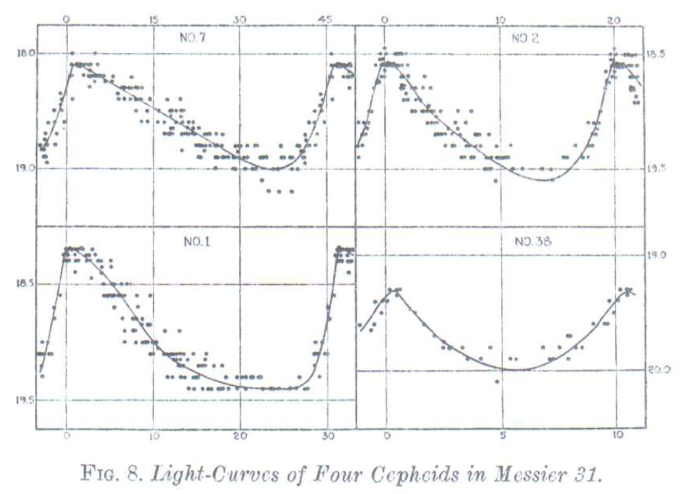
\includegraphics[width=0.8\textwidth]{Img/bertin_18.png}
\end{figure}

Noriamo che per le stelle più luminose il periodo è più lungo, mentre per quelle meno luminose è più breve; oltretutto, Hubble ricavò che esistono due tipi di Cefeidi, fatto che porta ad un errata misura delle dimensioni della stella. Supponiamo di avere una sola relazione in gioco, cioè che la luminosità apparente $L_ {app} \sim \frac{L}{R^2}$: dato che la luminosità è legata al periodo (in prima approssimazione, $L \propto \log T$) del quale è possibile ricavare una misura, possiamo dedurre la distanza $R$ della stella; in questo modo Hubble misurò distanze molto grandi ma errate di un fattore $2$: per esempio ricavò che la distanza di M31 era di $300 \, kpc$, mentre attualmente il valore riconosciuto è $770 \, kpc$.
\\
Una volta che conosciamo la distanza di una stella, come possiamo utilizzare tale dato per dedurre proprietà intriseche della stella? Dato che siamo in grado di misurarne la dimensione angolare, possiamo ricavare una stima del diametro $L \sim 1 \div 100 \, kpc$, anche se tale stima è affetta da errore poichè è difficile definire i contorni di una galassia (solitamente si considera la zona da cui proviene il $50 \%$ della luminosità); a questo punto, effettuando una proporzione con il Sole, possiamo stimare la massa di una galassia che è nell'ordine di $10^9 \div 10^{12} \, M_{\odot}$; possiamo infine ricavare il tempo dinamico $T_{din} \sim 10^8 \sim 10^9 \, yr$, dove $1 yr \sim \pi \cdot 10^7 \, s$.
\\
\begin{minipage}{.35\textwidth}
\centering
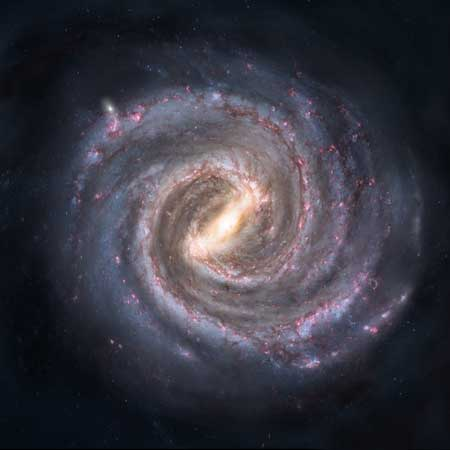
\includegraphics[width=1\textwidth]{Img/via_lattea.jpg}
\end{minipage}
\begin{minipage}{.65\textwidth}
\textbf{Alcuni dati numerici riguanti la Via Lattea}:
Massa: $M \sim 2 \cdot 10^{11} \, M_{\odot}$\\
La distanza del Sole dal centro della galassia è $R_{\odot} \sim 8 \, kpc$, mentre la velocità con cui ruota è $v_{\odot} \sim 220 \, \frac{km}{s}$, con un periodo di rotazione $T_{\odot} \sim 200 \cdot 10^6 \, yr$\\
La densità è $\Sigma \sim 50 \, M_{\odot}pc^{-2}$, che è circa la densità di un foglio di carta.\\
\end{minipage}

\vspace{0.2cm}

Possiamo inoltre calcolare l'accelerazione radiale del Sole, che vale $A_{r, \odot}= v_{\odot}^2 R_{\odot}^{-1}$. Se invece volessimo stimare l'acceerazione gravitazionale che il disco della galassia opera su una stella che si trova poco fuori dal disco stesso, possiamo ragionare come per una lastra carica elettricamente; ricaviamo allora $A_z = 2 \pi G \Sigma$.

Quello riportato a di seguito è detto \textbf{tuning fork diagram} per la sua forma che ricorda quella di un diapason; la paternità di tale grafico è attribuita ad Hubble, il quale quasi in contemporanea con le sue misure e osservazioni divise le galassie in tre principali forme: ellittiche, a spirale e a spirale barrata; in particolare, le galassie a spirale e a spirale barrata si distinguono da quelle ellittiche per la loro forma più schiacciata e per la presenza di un disco di rotazione, e al loro interno sono divise in tre sottocategorie indicate dalle lettere a, b, c. La Via Lattea si trova più o meno a metà fra le galassie di tipo Sb e SBb.

\begin{figure}[!h]
\centering
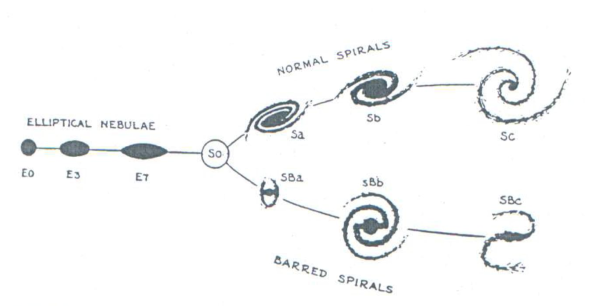
\includegraphics[width=0.8\textwidth]{Img/bertin_21.png}
\end{figure}

\vspace{0.5cm}

\section{Misure di massa}

Finora abbiamo dato un indicazione della massa di molti degli oggetti citati, e potremmo in realtà farlo per tutti gli oggetti celesti; la domanda che ci si pone allora è come faccia l'astronomo a ``pesare'' gli oggetti in cielo, cioè qual'è il procedimento per cui è possibile effettuare misure di massa. Prima di discutere questo punto, però, dobbiamo distinguere fra modello dinamico, cioè il modello con il quale descriviamo il nostro oggetto celeste, e ragionevole aspettazione, cioè quell'insieme di ipotesi su cui l'astronomo si basa e che devono essere adeguatamente giustificate.
\\
L'ipotesi base da cui partiamo è che i fotoni che vediamo sono emessi dalle stelle; infatti la quantità di gas ionizzato all'interno degli altri oggetti (ad esempio il mezzo interstellare, che compone la maggior parte della materia in un gruppo di stelle) è molto poca. Grazie a questo, possiamo dire che la luminosità e la massa della stella osservata sono legate da qualche relazione, e ragionevolmente tale relazione sarà lineare; siccome il Sole è una stella ``normale'', cioè non è una nana bianca o un altra stella particolare, possiamo utilizzarne i valori di massa e luminosità come unità di misura; avremo allora che per una stella con luminosità totale $\L$ possiamo scrivere:
$$\M=\frac{M_{\odot}}{L_{\odot}} \L$$

\chapter[Astrofisica osservativo-sperimentale]{Mennella-Cenni all'astrofisica osservativo-sperimentale}
\chapter[Astro-particelle]{Caccianiga-Le astro-particelle}
\chapter{Link utili}

\url{http://cosmo.fisica.unimi.it/didattica/corsi/introduzione-all-astrofisica/}\\
\url{www.eso.org}\\
\url{www.stsci.edu}\\
\url{sohowww.nascom.nasa.gov}\\
\url{adsabs.harvard.edu/abstract_service.html}\\
\url{arvix.org/archive/astro.ph}

\end{document}